%===============================================================================
% LaTeX sjabloon voor de bachelorproef toegepaste informatica aan HOGENT
% Meer info op https://github.com/HoGentTIN/bachproef-latex-sjabloon
%===============================================================================

\documentclass{bachproef-tin}

\usepackage{hogent-thesis-titlepage} % Titelpagina conform aan HOGENT huisstijl

%%---------- Documenteigenschappen ---------------------------------------------
% TODO: Vul dit aan met je eigen info:

% De titel van het rapport/bachelorproef
\title{Android zonder Google: Waarom je Google zou willen vermijden in je Android smartphone en hoe je het kan doen}

% Je eigen naam

\author{Casper Verswijvelt}

% De naam van je promotor (lector van de opleiding)
\promotor{Liesbeth Lewyllie}

% De naam van je co-promotor. Als je promotor ook je opdrachtgever is en je
% dus ook inhoudelijk begeleidt (en enkel dan!), mag je dit leeg laten.
\copromotor{Stein Desmet}


% Indien je bachelorproef in opdracht van/in samenwerking met een bedrijf of
% externe organisatie geschreven is, geef je hier de naam. Zoniet laat je dit
% zoals het is.
\instelling{---}

% De titel van het rapport/bachelorproef
\newcommand{\titel}{Android zonder Google: Waarom je Google zou willen vermijden in je Android smartphone en hoe je het kan doen}

% Datum van indienen (gebruik telkens de deadline, ook al geef je eerder af)
\newcommand{\datum}{31 mei 2019}

% Academiejaar
\academiejaar{2018-2019}

% Examenperiode
%  - 1e semester = 1e examenperiode => 1
%  - 2e semester = 2e examenperiode => 2
%  - tweede zit  = 3e examenperiode => 3
\examenperiode{2}

%===============================================================================
% Inhoud document
%===============================================================================

\begin{document}

%---------- Taalselectie -------------------------------------------------------
% Als je je bachelorproef in het Engels schrijft, haal dan onderstaande regel
% uit commentaar. Let op: de tekst op de voorkaft blijft in het Nederlands, en
% dat is ook de bedoeling!

%\selectlanguage{english}

%---------- Titelblad ----------------------------------------------------------
\inserttitlepage

%---------- Samenvatting, voorwoord --------------------------------------------
\usechapterimagefalse
%%=============================================================================
%% Voorwoord
%%=============================================================================

\chapter*{\IfLanguageName{dutch}{Woord vooraf}{Preface}}
\label{ch:voorwoord}

%% TODO:
%% Het voorwoord is het enige deel van de bachelorproef waar je vanuit je
%% eigen standpunt (``ik-vorm'') mag schrijven. Je kan hier bv. motiveren
%% waarom jij het onderwerp wil bespreken.
%% Vergeet ook niet te bedanken wie je geholpen/gesteund/... heeft

Ik zit vast in het Google ecosysteem. Dagelijks gebruik ik op mijn Android telefoon applicaties die door Google ontwikkeld zijn, en zo geef ik vrijwillig mijn data weg, die zij dan kunnen gebruiken om mij gerichte advertenties te sturen en God weet wat ze er nog allemaal mee doen. De applicaties die ze aanbieden zijn zo handig en makkelijk in gebruik, maar we stellen er ons geen vragen bij hoe Google deze services gratis kan aanbieden. 

Door de jaren heen kwam kwam ik steeds meer te weten over alle data die over mij werd verzameld, maar des te meer ik er van wist, des te meer dat ik er vrede mee nam. Ik zag dit onderwerp staan op het ideeënforum van HoGent, en wist direct dat dit een intressant onderwerp zou zijn, ook al is niet iets waar ik me persoonlijk toe in staat acht. Ik ben reeds te verwikkeld in hun praktijken, maar voor anderen is dit misschien nog niet te laat. Met dit onderzoek hoop ik mensen te informeren over de hoeveeld data die precies naar Google toe wordt gecommuniceerd, en wat de opties zijn om dit tegen te gaan.

Voor ik dit hoofdstuk afrond zou ik graag nog enkele mensen bedanken. Eerst en vooral zijn dit mijn ouders, die men te alle tijde hebben gesteund en door deze opleiding hebben gesleurd. Doorheen mijn studies probeerden ze me elke examenperiode tevergeefs van mijn uitstelgedrag af te helpen, wat ik heel erg appreciëer. Ten tweede wil ik mijn co-promotor, Stein Desmet, en mijn promotor, Liesbeth Lewyllie, bedanken. Ook zij wezen me tevergeefs op mijn uitstelgedrag, maar nog belangerijker is dat ze me tijdens het schrijven van dit werk continue constructieve feedback bezorgden. Ten slotte wil ik mijn trouwe Oneplus 5 bedanken, hoewel deze geen persoon is, voor mijn misbruik te toloereren en zich door mijn experimenten te sleuren zonder (al te veel) vast te lopen.

Dit gezegd zijnde, hoop ik dat jullie dit werk intressant vinden en dat deze informatie jullie helpt om een mening te vormen over de praktijken van Google.


%%=============================================================================
%% Samenvatting
%%=============================================================================

% De "abstract" of samenvatting is een kernachtige (~ 1 blz. voor een
% thesis) synthese van het document.
%
% Deze aspecten moeten zeker aan bod komen:
% - Context: waarom is dit werk belangrijk?
%  TODO- Nood: waarom moest dit onderzocht worden?
% - Taak: wat heb je precies gedaan?
% - Object: wat staat in dit document geschreven?
% - Resultaat: wat was het resultaat?
% - Conclusie: wat is/zijn de belangrijkste conclusie(s)?
% - Perspectief: blijven er nog vragen open die in de toekomst nog kunnen
%    onderzocht worden? Wat is een mogelijk vervolg voor jouw onderzoek?
%
% LET OP! Een samenvatting is GEEN voorwoord!

%%---------- Nederlandse samenvatting -----------------------------------------
%
% Als je je bachelorproef in het Engels schrijft, moet je eerst een
% Nederlandse samenvatting invoegen. Haal daarvoor onderstaande code uit
% commentaar.
% Wie zijn bachelorproef in het Nederlands schrijft, kan dit negeren, de inhoud
% wordt niet in het document ingevoegd.

\IfLanguageName{english}{%
\selectlanguage{dutch}
\chapter*{Samenvatting}
\lipsum[1-4]
\selectlanguage{english}
}{}

%%---------- Samenvatting -----------------------------------------------------
% De samenvatting in de hoofdtaal van het document

\chapter*{\IfLanguageName{dutch}{Samenvatting}{Abstract}}

Android telt de dag van vandaag reeds meer dan 2,5 miljard maandelijks actieve gebruikers. Android zelf is een zeer brede term. Deze bevat niet enkel het Android Open Source Project (AOSP), die de basisversie van het besturingssysteem omvat, maar ook alle aftakkingen hiervan. Zo'n aftakkingen worden vaak uitgebreid met extra functionaliteiten waarmee smartphone producenten zich proberen te onderscheiden van elkaar. Een ander softwarepakket dat vaak wordt meegeleverd met apparaten die bestemd zijn voor de westerse markt, maar niet inbegrepen is in het AOSP, is het 'Google Apps' pakket.

Google Apps, is niet, zoals de naam impliceert, enkel een verwijzing naar Google applicaties zoals Gmail, YouTube, Maps, etc. Hieronder valt ook het onderliggende 'Google Play Services' framework. Dit framework biedt API's aan die makkelijker te gebruiken zijn dan degene die in het AOSP te vinden zijn, en ook meer functionaliteiten aanbieden. Het 'Google Apps' softwarepakket staat apart van het besturingssysteem, en kan ook geüpdatet worden zonder dat het volledige besturingssysteem moet worden bijgewerkt. Zo kunnen applicatie-ontwikkelaars zeer makkelijk verderwerken met de nieuwste functionaliteiten die de Google Play Services aanbiedt, zelfs op apparaten die niet de laatste versie van Android bevatten.

Wanneer applicaties uit dit softwarepakket worden gebruikt, wordt er ook data verzameld over de gebruiker. Deze data gebruikt Google dan om gericht advertenties te kunnen sturen naar gebruikers. Volgens een onderzoek door \cite{schmidt_google-data-collection} is Android een essentiële factor bij Google's verzamelen van data. De producten die Google aanbiedt zijn in staat om gebruikersgegevens te verzamelen via een verscheidenheid aan technieken die door de doorsnee gebruiker mogelijk moeilijk te begrijpen zijn. Een groot deel van de verzamelde data wordt verzameld wanneer de gebruiker niet rechtstreeks in contact komt met Google's producten. 

Applicaties binnen dit softwarepakket worden, wanneer deze wordt meegeleverd met het besturingssysteem, geïnstalleerd als systeemapplicaties. Dit betekent dat ze nooit volledig verwijderd kunnen worden. Dit wordt een probleem wanneer de gebruiker wil beperken welke Google software er zich op zijn/haar apparaat bevindt. Google zelf biedt reeds enkele opties aan om het verzamelen van data in te perken, maar deze zijn beperkt.

Er werd reeds onderzocht hoeveel een standaard ingesteld Android apparaat communiceert met Google, maar dit werd nog niet toegepast samen met verschillende 'ontgoogle' methodes. In dit onderzoek werd onderzocht wat de mogelijke manieren zijn om Google zoveel mogelijk te verbannen van het apparaat, beide door methoden die Google zelf aanbiedt en methoden die niet rechtstreeks door Google ondersteund worden. Hieruit kwamen drie testgevallen voort: Android met fabrieksinstellingen, Android met aangepaste instellingen en een volledig aangepaste versie van Android. Bij elk testgeval werd bekeken welke stappen moesten worden gevolgd om de gewenste toestand van het testgeval te bereiken. Hierna werd er per geval geanalyseerd hoeveel keer er naar Google gecommuniceerd werd, zonder dat er enige interactie met het apparaat plaatsvond. 

Uit de resultaten van dit experiment bleek dat er per uur gemiddeld 20 keer naar Google werd gecommuniceerd wanneer het Android apparaat is ingesteld volgens de standaard instellingen. Het aantal verzonden verzoeken in deze toestand was zeer uiteenlopend wanneer dit werd vergeleken met de resultaten van het experiment bij de andere testgevallen. Dit aantal lag hier minimum op 4 verzoeken per uur en maximum op 36.

In het geval waar Google zoveel mogelijk werd ingetoomd door middel van de opties aangeboden door Google en Android te gebruiken, werd er gemiddeld 3 keer per uur naar Google toe gecommuniceerd. Dit aantal ligt direct een stuk lager dan het voorgaande experiment, en met een minimum van 2 verzoeken en een maximum van 6 verzoeken zijn deze resultaten ook veel minder uiteenlopend. Tegenover het voorgaande testgeval werd het aantal verzoeken met 85\% gereduceerd. De stappen die moesten worden gevolgd om dit resultaat te bekomen, waren niet direct intuïtief te vinden binnen het Android besturingssysteem, maar eens gevonden zijn ze makkelijk aan te passen.

In het laatste geval werd er op het testapparaat een andere versie van Android geïnstalleerd, die geen enkele extra software van Google bevat, namelijk LineageOS. De stappen die hiervoor moesten gevolgd worden, waren alles behalve gebruiksvriendelijk. De benodigdheid van extra software die niet op een centrale plek op het internet wordt aangeboden is mogelijk een struikelblok voor gebruikers indien ze deze methode zelf ook willen toepassen. De stappen moeten zeer specifiek opgevolgd worden en de mogelijkheid dat het apparaat in een onbruikbare staat terechtkomt, is reëel. De moeite wordt wel beloond, want uit de resultaten blijkt doorheen alle uitvoeringen van het experiment dat er geen enkele communicatie met Google voorkomt in deze toestand.

Binnen dit onderzoek werd de inhoud en specifieke URL van aanvragen naar Google niet geanalyseerd. De inhoud van deze aanvragen kan echter wel meer licht laten schijnen op welke informatie er precies wordt gecommuniceerd naar Google toe. Verder kan het ook interessant zijn dit experiment toe te passen op een 'day-in-the-life' scenario om zo een meer realistische werklast op het apparaat uit te oefenen.


%---------- Inhoudstafel -------------------------------------------------------
\pagestyle{empty} % Geen hoofding
\tableofcontents  % Voeg de inhoudstafel toe
\cleardoublepage  % Zorg dat volgende hoofstuk op een oneven pagina begint
\pagestyle{fancy} % Zet hoofding opnieuw aan

%---------- Lijst figuren, afkortingen, ... ------------------------------------

% Indien gewenst kan je hier een lijst van figuren/tabellen opgeven. Geef in
% dat geval je figuren/tabellen altijd een korte beschrijving:
%
%  \caption[korte beschrijving]{uitgebreide beschrijving}
%
% De korte beschrijving wordt gebruikt voor deze lijst, de uitgebreide staat bij
% de figuur of tabel zelf.

\listoffigures
\listoftables
% Als je een lijst van afkortingen of termen wil toevoegen, dan hoort die
% hier thuis. Gebruik bijvoorbeeld de ``glossaries'' package.
% https://www.overleaf.com/learn/latex/Glossaries

%---------- Kern ---------------------------------------------------------------

% De eerste hoofdstukken van een bachelorproef zijn meestal een inleiding op
% het onderwerp, literatuurstudie en verantwoording methodologie.
% Aarzel niet om een meer beschrijvende titel aan deze hoofstukken te geven of
% om bijvoorbeeld de inleiding en/of stand van zaken over meerdere hoofdstukken
% te verspreiden!

%%=============================================================================
%% Inleiding
%%=============================================================================

\chapter{\IfLanguageName{dutch}{Inleiding}{Introduction}}
\label{ch:inleiding}

%TODO inleiding inleiding

%De inleiding moet de lezer net genoeg informatie verschaffen om het onderwerp te begrijpen en in te zien waarom de onderzoeksvraag de moeite waard is om te onderzoeken. In de inleiding ga je literatuurverwijzingen beperken, zodat de tekst vlot leesbaar blijft. Je kan de inleiding verder onderverdelen in secties als dit de tekst verduidelijkt. Zaken die aan bod kunnen komen in de inleiding~\autocite{Pollefliet2011}:

%\begin{itemize}
%  \item context, achtergrond
%  \item afbakenen van het onderwerp
%  \item verantwoording van het onderwerp, methodologie
%  \item probleemstelling
%  \item onderzoeksdoelstelling
%  \item onderzoeksvraag
%  \item \ldots
%\end{itemize}

\section{\IfLanguageName{dutch}{Probleemstelling}{Problem Statement}}
\label{sec:probleemstelling}

Er is reeds veel sprake over hoeveel data Google daadwerkelijk bijhoudt over zijn gebruikers en waarom dit voor de gebruiker zelf ook negatief kan zijn. Deze data wordt verzameld wanneer men gebruik maakt van Google services die standaard meegeleverd zijn in een Android telefoon. Deze Google services zijn onder meer applicaties zoals Google Play Store, Google Maps, YouTube, etc. Ook onderliggende frameworks aangeboden door Google die andere applicaties kunnen gebruiken, horen hierbij. 

Het probleem ligt hier bij het feit dat de gebruikers van deze services niet voldoende weten waarom deze data wordt bijgehouden, wat er mee gedaan wordt en waarom ze dit misschien beter zouden voorkomen. Denk in dit verband ook aan de GDPR-wetgeving die eveneens werd ingevoerd in functie van het beter informeren van de Europese burger over welke data er over hem/haar wordt opgeslagen \footnote{\url{https://gdpr-eu.be/wat-is-gdpr/}}. Google werd begin 2019 ook reeds bestraft in Frankrijk voor het overtreden van deze wetgeving \autocite{Boete2019}. Het artikel door \cite{LaurensVerhagen2019} vermeldt dat techgiganten hun dominante machtspositie misbruiken om zo zeer grote hoeveelheden informatie over hun gebruikers te weten te komen. Op deze manier kunnen ze surrealistische hoeveelheden geld verdienen met gegevens van consumenten \autocite{propken_google-data}. 

Dit werk richt zich dan ook naar Android gebruikers die belang hechten aan hun privacy, en heeft als doel hun beter te informeren.

%Uit je probleemstelling moet duidelijk zijn dat je onderzoek een meerwaarde heeft voor een concrete doelgroep. De doelgroep moet goed gedefinieerd en afgelijnd zijn. Doelgroepen als ``bedrijven,'' ``KMO's,'' systeembeheerders, enz.~zijn nog te vaag. Als je een lijstje kan maken van de personen/organisaties die een meerwaarde zullen vinden in deze bachelorproef (dit is eigenlijk je steekproefkader), dan is dat een indicatie dat de doelgroep goed gedefinieerd is. Dit kan een enkel bedrijf zijn of zelfs één persoon (je co-promotor/opdrachtgever).

\section{\IfLanguageName{dutch}{Onderzoeksvraag}{Research question}}
\label{sec:onderzoeksvraag}

Dit werk zal bespreken of en hoe het kan vermeden worden dat de gebruiksdata van Android gebruikers wordt verzameld, en hoe dit kan gerealiseerd worden door Google zoveel mogelijk, al dan niet volledig, te verbannen uit hun smartphone.

Concreet zal er onderzocht worden via welke methodes dit kan gedaan worden, en hoe het uitvoeren van deze methodes gereflecteerd wordt in de data die uiteindelijk nog steeds naar Google gecommuniceerd wordt.
%Wees zo concreet mogelijk bij het formuleren van je onderzoeksvraag. Een onderzoeksvraag is trouwens iets waar nog niemand op dit moment een antwoord heeft (voor zover je kan nagaan). Het opzoeken van bestaande informatie (bv. ``welke tools bestaan er voor deze toepassing?'') is dus geen onderzoeksvraag. Je kan de onderzoeksvraag verder specifiëren in deelvragen. Bv.~als je onderzoek gaat over performantiemetingen, dan 

\section{\IfLanguageName{dutch}{Onderzoeksdoelstelling}{Research objective}}
\label{sec:onderzoeksdoelstelling}

Het doel van dit onderzoek is om een beeld te geven van de mogelijkheden waartoe Android gebruikers beschikken om Google zo veel mogelijk te vermijden, en hoe effectief deze methoden zijn. De effectiviteit zal worden gemeten aan de hand van een beschrijving van data die wordt gecommuniceerd in een bepaalde toestand van een Android apparaat. Wanneer uit deze resultaten kan opgemaakt worden dat de gebruikte methodes wel degelijk een impact hebben op de hoeveelheid van  gecommuniceerde data, is dit onderzoek succesvol.
%Wat is het beoogde resultaat van je bachelorproef? Wat zijn de criteria voor succes? Beschrijf die zo concreet mogelijk.

\section{\IfLanguageName{dutch}{Opzet van deze bachelorproef}{Structure of this bachelor thesis}}
\label{sec:opzet-bachelorproef}

% Het is gebruikelijk aan het einde van de inleiding een overzicht te
% geven van de opbouw van de rest van de tekst. Deze sectie bevat al een aanzet
% die je kan aanvullen/aanpassen in functie van je eigen tekst.

De rest van deze bachelorproef is als volgt opgebouwd:

In hoofdstuk~\ref{ch:stand-van-zaken} wordt een overzicht gegeven van de stand van zaken binnen het onderzoeksdomein, op basis van een literatuurstudie.

In hoofdstuk~\ref{ch:methodologie} wordt de methodologie toegelicht en worden de gebruikte onderzoekstechnieken besproken om een antwoord te kunnen formuleren op de onderzoeksvragen.

In hoofdstuk~\ref{ch:resultaten} zullen de resultaten worden besproken die volgden uit de experimenten van hoofdstuk \ref{ch:methodologie}.

In hoofdstuk~\ref{ch:conclusie}, tenslotte, wordt de conclusie gegeven en een antwoord geformuleerd op de onderzoeksvragen. Daarbij wordt ook een aanzet gegeven voor toekomstig onderzoek binnen dit domein.
\chapter{Stand van zaken}
\label{ch:stand-van-zaken}

% Tip: Begin elk hoofdstuk met een paragraaf inleiding die beschrijft hoe
% dit hoofdstuk past binnen het geheel van de bachelorproef. Geef in het
% bijzonder aan wat de link is met het vorige en volgende hoofdstuk.

% Pas na deze inleidende paragraaf komt de eerste sectiehoofding.

Om de verschillende 'ontgoogle' manieren met elkaar te kunnen vergelijken, moeten we eerst wat dieper ingaan op de verschillende Google componenten die te vinden zijn binnen het Android besturingssysteem en hoe deze zoveel mogelijk te limiteren en/of uit te schakelen zijn. In dit hoofdstuk zult u meer te weten komen over wat er precies gebeurt achter de schermen van Android en hoe pecies een 'ontgoogling' kan gebeuren.

\section{Google componenten binnen Android}
%TODO voornamelijk weg, niet waterdicht genoeg
Google software binnen het Android besturing bestaat voornamelijk uit de 'Google Play-Services', het achterliggende 'brein' van Google, en Google applicaties, zoals GMail, Google Play Store, etc.

\subsection{Google Play-Services}

Aan het hart van het Android besturingssysteem liggen de 'Google Play-Services'. Deze services zijn zeer nauw met het Android besturingssysteem geïntegreerd, en bieden een bundel van API's aan. \autocite{marshall_google-play-services}. Een API of 'Application Program Interface' is kort gezegd een set van hulpmiddelen die het voor applicatie-ontwikkelaars makkelijker maakt om applicaties te ontwikkelen. \autocite{beal_api}

AOSP, ook gekend als Android Open Source Project, is de basis van het Android besturingssysteem. Zoals de naam zelf al zegt, is dit project volledig 'open-source'. Dit houdt in dat iedereen vrij is om de broncode te gebruiken en aan te passen. 

De Android versie die in de meeste gevallen op mensen hun smartphone draait, is echter niet volledig 'open-source' maar ook voor een deeltje 'closed-source'. Smartphone producenten voeren vaak nog wijzigen door op AOSP, die invloed hebben op hoe visuele elementen er uitzien, extra functionaliteiten toevoegen en zorgen dat alle hardware die gebruikt wordt binnen het apparaat ook ondersteund wordt door apparaat-specifieke drivers. Zo ontwikkelt Xiaomi voor hun apparaten een eigen versie van Android die ze MIUI noemen, OnePlus ontwikkelt een eigen versie van Android die ze OxygenOS noemen, LG heeft LG UX, etc. Voor de westerse markt worden de Google Apps vaak opgenomen in het besturingssysteem. Google zelf biedt ook Android telefoons aan, zoals de reeds verouderde 'Nexus' apparaatlijn en de huidige 'Pixel' apparaatlijn. Zelf het besturingsysteem dat op deze apparaten draait is niet onaangepast, ook al wordt deze vaak als de 'schoonste' versie van Android beschouwd. Binnen hun versie van Android zijn ook de gepatenteerde Google Apps aanwezig \autocite{torres_stockandroid}. Steeds meer producenten bieden apparaten aan met een zo min mogelijk aangepaste versie van Android, om zo beroep te doen op mensen die op zoek zijn naar de 'stock experience'. Via het 'Android One' programma dat Android aanbiedt, is het ook makkelijker voor producenten om dit aan te bieden. Ook hierin zijn Google Apps inbegrepen. \autocite{android_androidone}.  Dit deel omvat dan alle applicaties van Google zelf, bv. GMail, Google Maps, en de onderliggende 'Google Play-Services' \autocite{amadeo_open-source}.

AOSP biedt een bundel API's  aan, maar Google zelf adviseert om de API's van de Google Play-Services te gebruiken. Deze zijn immers een stuk makkelijker te gebruiken zijn, en zorgen ervoor dat applicaties niet rechtstreeks afhankelijk zijn van Android besturingssysteem updates. Deze API's, zijn dan ook 'closed-source', tegenover de API's van AOSP, die 'open-source' zijn \autocite{marshall_google-play-services} . 

Een voorbeeld hiervan is de locatie service. AOSP biedt een 'Location API' aan. Wanneer een applicatie gebruik maakt van deze API, moet er expliciet gekozen worden tussen 3 'location providers'. Elk van deze gebruikt een verschillende manier om de locatie van een gebruiker te bepalen \autocite{android_location-strategies}. De GPS provider gebruikt de fysieke GPS chip binnen het apparaat, en kan hierdoor ook de meest accurate locatiegegevens teruggeven, maar deze verbruikt ook het meeste energie. De netwerk provider maakt gebruik van de GPS chip, samen met gegevens van het mobiele netwerk om zo een snelle initiële verbinding te krijgen. De nauwkeurigheid van de locatiegegevens die hier worden teruggeven is lager, maar deze methode zorgt wel voor een lager energieverbruik. Tenslotte is er ook de passieve provider. Deze zal, in tegenstelling tot de andere providers, niet actief zoeken naar een verbinding. In plaats daarvan, maakt deze gebruik van locatiegegevens die verschaft werden door de andere providers, wanneer deze door andere applicaties worden aangesproken \autocite{idris_location-providers}. De Google Play Serivces Location API heeft als voordeel dat ontwikkelaars niet expliciet meer moeten kiezen tussen één van deze drie providers. Deze keuze wordt automatisch gemaakt zodat nauwkeurigheid en energieverbruik geoptimaliseerd wordt. \autocite{android_location-strategies}

\blockcquote{android_location-strategies}{
    The Google Location Services API, part of Google Play Services, provides a more powerful, high-level framework that automatically handles location providers, user movement, and location accuracy. It also handles location update scheduling based on power consumption parameters you provide. In most cases, you'll get better battery performance, as well as more appropriate accuracy, by using the Location Services API.
}

Steeds meer en meer open-source applicaties, die voorheen te vinden waren binnen AOSP, worden achtergelaten en vervangen door een closed-source versie op de Google Play Store, de applicatie van Google waarmee gebruikers applicaties kunnen downloaden en installeren. Ook de Play Store maakt gebruik van de Google Play-Services om applicaties automatisch te kunnen updaten. Op deze manier probeert Google haar eigen applicaties zoveel mogelijk macht te geven tegenover de 'open-source' applicaties binnen AOSP. \autocite{amadeo_open-source}

Doordat zeer veel applicaties dus rechtstreeks afhangen van de Google Play-Services, zullen veel applicaties ook regelrecht niet meer zoals gewenst functioneren wanneer de Play-Services niet aanwezig zijn of deze niet beschikt over de nodige toestemmingen \autocite{marshall_google-play-services}. Android handhaaft een toestemmingssysteem waarbij elke applicatie eerst toestemming moet vragen voordat deze aan gevoelige gebruikersdata kan. Voorbeelden van dergelijke machtigingen zijn toegang tot de camera, contacten en SMS informatie \autocite{android_permissions}. Standaard krijgt Google Play Services, als enige applicatie, alle machtigingen toegekend, zoals te zien in figuur \ref{fig:permissions1}. Wanneer er geprobeerd word om hier de machtigingen in te perken, wordt er ook gemeld dat dit kan leiden tot het verstoren van basisfunctionaliteiten, zoals te zien in figuur \ref{fig:permissions1}. \textquote{Als je deze machtiging weigert, kan het zijn dat basisfuncties van je apparaat niet meer werken zoals bedoeld.}.

\begin{figure}
    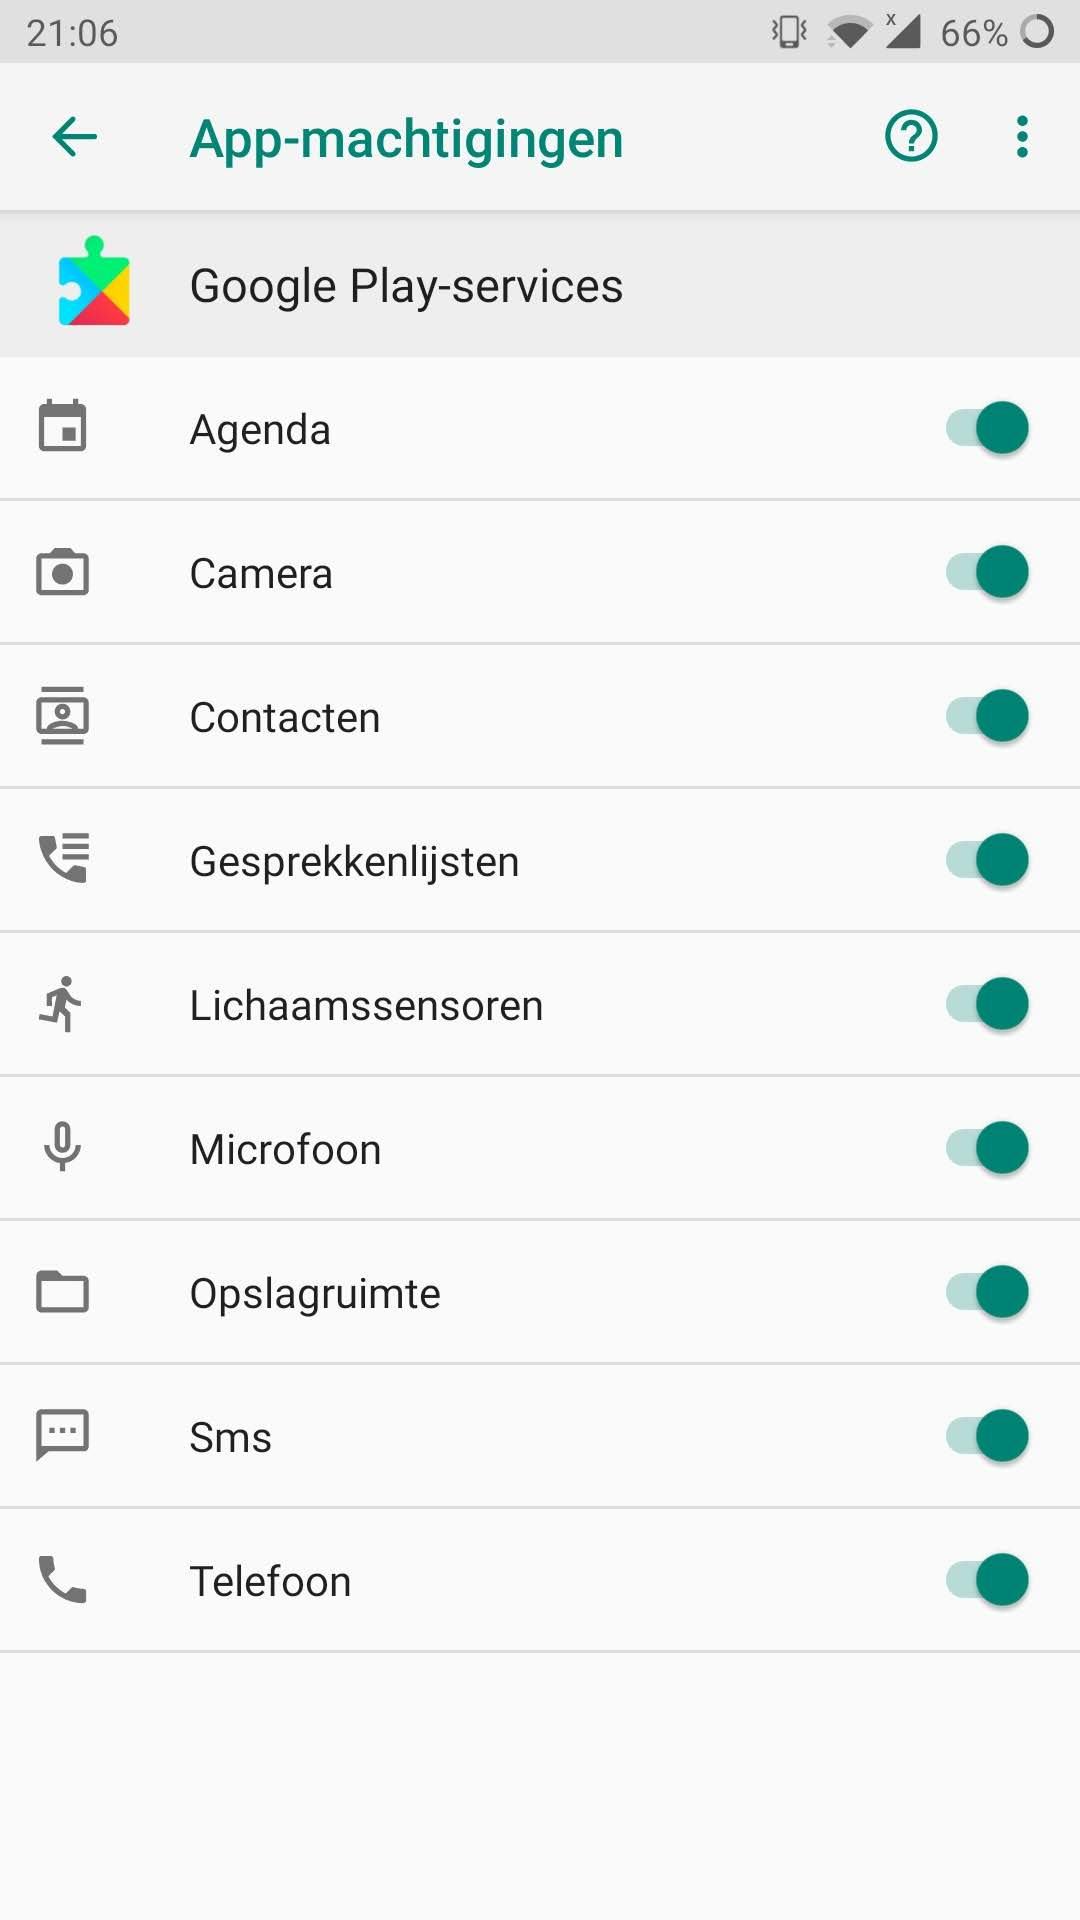
\includegraphics[width=0.4\textwidth]{img/machtigingen.jpg}
    \caption{Screenshot van vereiste machtigingen van Google Play Services}
    \label{fig:permissions1}
\end{figure}

\begin{figure}
    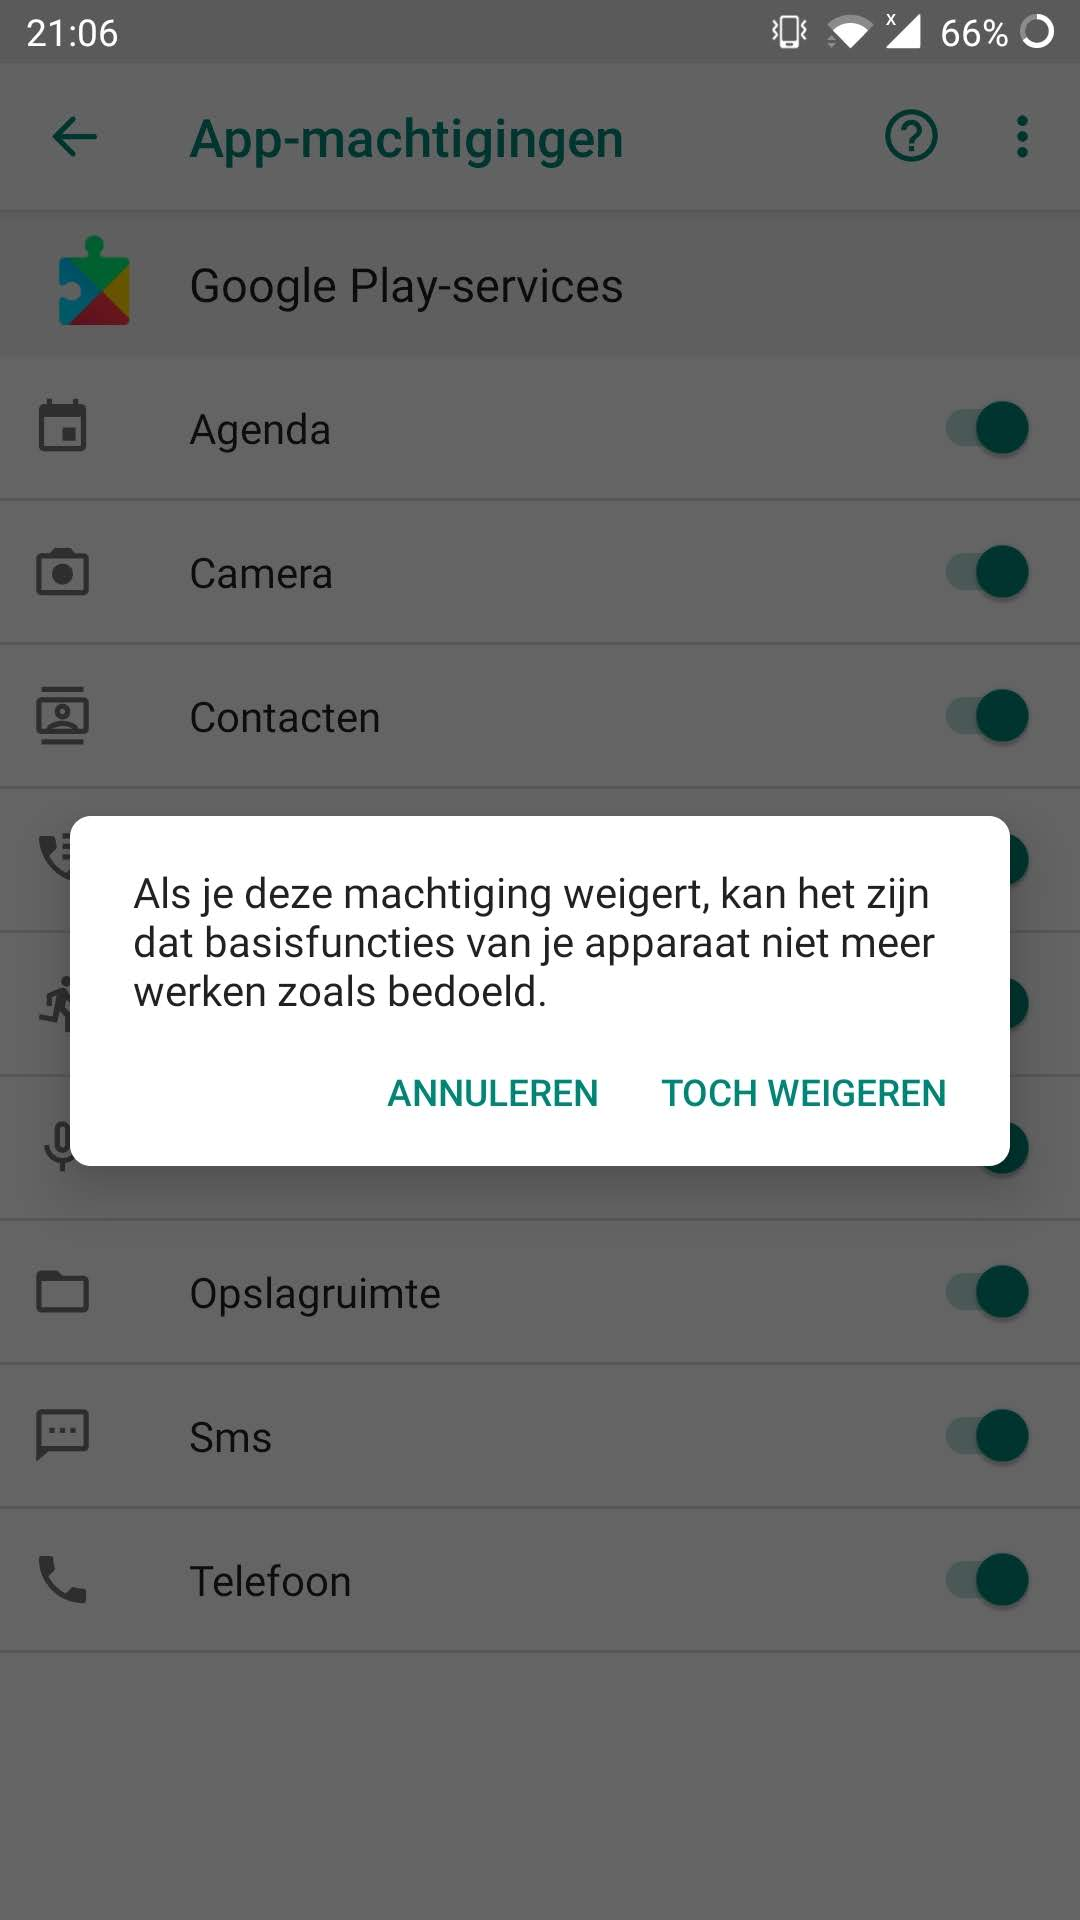
\includegraphics[width=0.4\linewidth]{img/machtigingen_melding.jpg}
    \caption{Screenshot van melding bij inperken van machtigingen van Google Play Services}
    \label{fig:permissions2}
\end{figure}

\subsection{Google Applicaties}

Een ander Google component binnen Android zijn alle Google applicaties. Afhankelijk van de fabrikant van de smartphone, zal er een heel pakket aan Google applicaties samen met de Google Play-Services, al dan niet geïnstalleerd zijn. Google applicaties zijn als systeem-applicaties geïnstalleerd, wat betekent dat ze zonder software aanpassingen niet van  het apparaat kunnen verwijderd worden. Wel is het mogelijk om deze applicaties 'uit te schakelen'. Dit houdt in dat ze niet meer op de achtergrond kunnen worden uitgevoerd, en dus ook geen meldingen kunnen sturen.

Applicaties die hier binnenvallen zijn GMail, Google, Google Play Films, Google Play Store, etc.

\section{Mogelijke ontgoogle manieren}

Het doel van het ontgooglen is dan om de Google software zodanig te vermijden zodat je op  een zo min mogelijke manier nog vastzit aan Google. Dit kan mogelijks op enkele manieren gebeuren, die zullen worden besproken in volgende subsecties.

\subsection{Zachte ingrepen}

Onder zachte ingrepen verstaan we de methoden die enkel gebruik maken van opties die ons rechstreeks door Android of Google worden aangeboden, zonder softwarematige wijzigingen aan te brengen aan het besturingssysteem.

\subsubsection{Verwijderen van Google account op het apparaat}

Gebruik van een Google account word aangeraden bij het gebruik van een Android telefoon, maar is niet verplicht. Bij het instellen van het Android besturingssysteem kunt u de stap om in te loggen bij Google gewoon overslaan. Het is ook mogelijk om een ingelogde Google account later te verwijderen. Enkele applicaties zullen niet werken of gelimiteerde functionaliteit hebben hierdoor, maar mogelijk wilt u deze Google applicaties niet gebruiken als u als doel 'ontgooglen' hebt.

\subsubsection{Niet gebruiken van Google applicaties}
Door Google applicaties regelrecht niet te gebruiken, is de grip van Google op Android telefoons al direct een heel stuk zwakker.
Zoals eerder al gezegd, is het niet mogelijk om Google applicaties te verwijderen aangezien ze geïnstalleerd zijn als systeem-applicaties. Ze kunnen echter wel uitgeschakeld worden. Door Google applicaties niet te gebruiken missen we wel redelijk wat basisfunctionaliteiten. De applicaties die dan worden misgelopen, zijn onder andere Google Maps (online kaartendienst), GMail (mail client), Google Foto's (applicatie om foto's bij te houden en te synchroniseren met de cloud), Chrome (internetbrowser), YouTube (online videoplatform), Google Calendar (agenda applicatie), Google Keyboard (toetsenbord), Google Play Store (app-store), etc.  Gelukkig biedt het internet meer dan genoeg alternatieven voor elke Google applicatie. Deze methode zorgt er niet voor dat Google van het besturingssysteem verbannen wordt en het apparaat zal nog steeds communiceren met Google.

\subsubsection{Uitschakelen van persoonlijke advertenties}
Een mogelijkheid die Google ons geeft, is het uitschakelen van persoonlijke advertenties. Door gebruik te maken van een 'advertising ID' kan Google externen toegang geven tot gebruikersinformatie zoals locatie en apps die gebruikt worden. Google geeft ons de mogelijkheid om toegang tot deze 'advertising ID' uit te schakelen. Dit kan een gebruiker doen door eerst naar het instellingen menu te navigeren, 'Google' te selecteren, en vervolgens 'Advertenties' te selecteren. Hier kan je je door middel van een schuifbalkje afmelden voor personalisatie van advertenties. \autocite{knight_degoogle}

\subsubsection{Veranderen van de standaard DNS server}
Een DNS server is een server, die wanneer je naar een bepaalde site surft, de vertaalstap maakt tussen een domein en het IP adres van de bijhorende webruimte. Als de DNS server van een Android smartphone is ingesteld op de DNS server van Google, kan google uw surfgedrag opvolgen om zo een profiel op te bouwen voor adverteerders. Door de DNS server aan te passen naar één van uw provider of andere aanbieder, kunt u dit voorkomen.

Tot Android 8.0, ook wel gekend als Android Oreo, was er geen mogelijkheid om de DNS server bij gebruik van het mobiele netwerk aan te passen, en enkel gelimiteerde mogelijkheden om deze aan te passen bij gebruik van Wi-Fi. Er bestaan echter wel applicaties die door middel van een 'omleiding' en het gebruik van de VPN functie op Android toch hetzelfde resultaat kunnen bekomen \autocite{knight_degoogle}. 

Sinds Android 9.0, ook wel gekend als Android Pie, bestaat DNS-over-TLS. In de instellingen van een Android telefoon kan deze instelling gevonden worden onder 'Wi-FI \& internet' en vervolgens 'Privé-DNS'. Hier kan systeem-wijd een privé-DNS-provider worden ingesteld. Bij het gebruiken van deze functie wordt door middel van encryptie de beveiliging en privacy tussen de client en de DNS-server verbeterd. \autocite{google_dns-tls}

\subsection{Harde ingrepen}

Onder harde ingrepen verstaan we de methoden die gebruik maken van software aanpassingen om zo Google zo veel mogelijk te verbannen.

\subsubsection{Installeren van een Custom ROM}
Een 'Custom Android ROM' verwijst naar de versie van AOSP waarop een bepaalde smartphone draait \autocite{custom-rom}. De versie van Android die vooraf geïnstalleerd is op een smartphone wordt de 'stock ROM' genoemd. De meeste stock ROM's bevatten standaard reeds de Google Play-Services en bijhorende Google applicaties, maar dit is zeker geen vereiste voor het android besturingssysteem. In China is het gebruik van Google verboden, en bijgevolg bevatten toestellen die bedoeld zijn voor de Chinese markt geen enkele verwijzing naar Google software. Doordat de Google Play Store niet kan werken zonder de Google Play-Services, moeten chinese bedrijven een eigen 'app store' implementeren om deze te vervangen. Hetzelfde is waar voor custom ROM's. De ontwikkelaar kan zelf kiezen of hij/zij google software wilt meeleveren in zijn versie van het besturingssysteem.

Om een custom ROM te installeren, zijn er wel enkele vereisten waaraan een apparaat moet voldoen. Ten eerste moet het apparaat beschikken over een 'unlocked bootloader'. Standaard wordt een Android apparaat geleverd met een 'locked bootloader'. Het hangt dan af van de fabrikant hoe het al dan niet mogelijk is om deze bootloader te unlocken. Het proces om dit te doen verschilt van fabrikant tot fabrikant, en bij meeste fabrikanten houdt dit proces ook in dat alle data op het apparaat wordt gewist. De tweede vereiste om een custom ROM te kunnen installeren is dat er 'custom recovery' geïnstalleerd is. Dit is een gelimiteerde opstartmodus die ons toelaat om de 'custom ROM' te installeren \autocite{hoffman_custom-recovery}.

Als er binnen de custom ROM geen Google software te vinden is, kan een Android telefoon die deze versie van het besturingssysteem draait als 'ontgoogelt' beschouwd worden. Dit betekent echter niet dat alle functionaliteiten die voordien werkten, nog steeds allemaal zullen werken. Wanneer applicatie-ontwikkeleraars kiezen om tijdens de ontwikkeling verder te werken met een API die wordt aangeboden door de Google Play-Services, en niet op een API van AOSP, dan zal deze applicatie hoogstwaarschijnlijk niet werken naar behoren, of zelfs direct crashen wanneer deze geopend wordt.


Desalniettemin, bestaat er een open-source implementatie van de Google Play-Services, genaamd microG. Wanneer deze geïnstalleerd wordt bovenop een Google-loze custom ROM, zou het grootste deel van de verloren functionaliteiten hersteld worden. De motivatie voor dit project staat zeer duidelijk uitgelegd op hun site, en luidt als volgt. \blockcquote{microg}{
    The linux-based open-source mobile operating system Android is not only the most popular mobile operating system in the world, it’s also on the way to becoming a proprietary operating system. How is that?
    
    While the core operating system is still released as part of the Android Open Source Project, the majority of core apps are not. It gets worse: More and more libraries and APIs are only available on phones that run various Google apps pre-installed, effectively locking third-party apps to the Google ecosystem. For these reasons Android is described as being a “look but don’t touch” kind of open.
    
    At this point, several popular open-source applications already require some of Google’s proprietary libraries to be installed. Increasing demand in the free software community in addition to severe problems in Google’s proprietary software discovered by the Android modding community, have led to the development of a free software clone of Google’s proprietary core libraries and applications - the microG Project was born.
    
    Although most microG components are far from complete, users are amazed by the results. Free software users got extended application support, privacy-caring users can reduce or monitor data that is sent to Google and especially older phones can expect some battery life improvements. microG is not only used on real devices, but also replaces Google tools in test emulators and is even used in virtual mobile infrastructure.
}
Zoals hierboven vermeld, probeert microG een vervanging te zijn voor de gesloten software van Google, de Google Play-Services. Ook wordt er gezegd dat de implementatie van de microG componenten verre van compleet zijn. Het feit dat microG de functionaliteit van de Google Play-Services wilt nabootsen, impliceert ook dat de nieuwste functies niet direct beschikbaar zullen zijn binnen dit alternatief. Naarmate de ontwikkelaar-gemeenschap achter dit project blijft groeien zal deze functionele achterstand wel inkrimpen.

MicroG maakt het mogelijk om terug de Google Play Store te gebruiken, maar biedt ook een aparte applicatie aan genaamd 'FakeStore'. Deze zorgt ervoor dat andere applicaties denken dat de Play Store aanwezig is, terwijl dit natuurlijk niet zo is. Verder biedt deze applicatie niets van functionaliteit. Alternatieve app-stores zoals F-Droid of de Yalp Store zijn ook mogelijke opties. \autocite{shadow53_play-store}

\paragraph*{SafetyNet}

Aan bovenstaande methode zijn er ook negatieve kanten. Android heeft namelijk veiligheidsmaatregelen getroffen met betrekking tot het blokkeren van veiligheidsrisico's, 'sjoemelen' met het apparaat, kwaadaardige applicaties en 'nep' gebruikers \autocite{android_safetynet}. Dit systeem heet SafetyNet, en maakt deel uit van de Google Play Services. App-ontwikkelaars kunnen via de SafetyNet Attestation API nagaan op welk niveau aan de systeem integriteits controle voldaan wordt. Op basis van deze informatie kunnen bepaalde functies binnen de applicatie geblokkeerd worden. Het is ook mogelijk dat de volledige applicatie onbruikbaar wordt. Denk hier bijvoorbeeldt aan het bekende spel 'Pokemon GO', die het spel onspeelbaar maakt op apparaten die niet aan de SafetyNet controle voldoen. In de Belfius mobiele bankier-applicatie is het bijvoorbeeld niet mogelijk om vingerafdruk-authenticatie te gebruiken op zo'n apparaten. Ook de Play Store kan op basis van deze data het installeren van specifieke applicaties volledig voorkomen.

Wanneer er een custom ROM geïnstalleerd is, is de bootloader ook ontgrendelt. Aan de hand van de CTS (Compatibility Test Suite) kan Google bekijken of er ook maar enige aanpassingen zijn toegepast op het systeem. Een unlocked bootloader valt hier ook onder.





%%=============================================================================
%% Methodologie
%%=============================================================================

\chapter{\IfLanguageName{dutch}{Methodologie}{Methodology}}
\label{ch:methodologie}

Binnen dit experiment zullen er concreet 3 specifieke toestanden van een Android apparaat met elkaar vergeleken worden. Het eerste geval is een Android apparaat waarop er nog geen enkele wijziging is doorgevoerd. Deze staat dus nog gelijk met de fabrieksinstellingen van het apparaat. Bij het tweede geval zijn de instellingen zo aangepast dat de dataverzameling van Google geminimaliseerd wordt. Bij deze toestand wordt er optimaal gebruik gemaakt van de mogelijkheden die Google en het Android besturingssysteem bieden zodat er zo min mogelijk data wordt verzameld. In het derde geval zullen er methodes gebruikt worden, die niet direct door Google of Android zelf worden ondersteund, om zo Google volledig te proberen elimineren van het apparaat.

Bij deze drie gevallen zal er in detail beschreven worden welke stappen precies moeten worden genomen om de testtoestand van het apparaat te bekomen. Daarna zal het internetverkeer van elk geval geanalyseerd worden gedurende 1 uur. Concreet wordt er hier geregistreerd hoeveel keer er gemiddeld data wordt verstuurd naar domeinen van Google.

\section{Testapparaat}
\label{sec:testapparaat}
Het experiment zal plaatsvinden op een Oneplus 5 apparaat (model nr. ONEPLUS A5000). Dit apparaat draait op een aangepaste versie van Android, genaamd OxygenOS. OxygenOS is een Android ROM die gekend is voor het toevoegen van configureerbaarheid en handige functies, terwijl de 'look and feel' grotendeels gelijk blijft in vergelijking met stock Android. De bloatware die hierbinnen wordt meegeleverd is ook minimaal. De laatste versie van OxygenOS die beschikbaar is op het moment van schrijven, is OxygenOS 9.0.5, die voortbouwt op Android 9.0, ofwel Android Pie.

\section{Testgevallen}
\label{sec:testgevallen}

In deze sectie zullen de verschillende testgevallen in detail besproken worden.

\subsection{Testgeval 1: Android met fabrieksinstellingen}
\label{sec:testgeval1}
Binnen dit geval zal gebruik gemaakt worden van een Android apparaat waarbij buiten de initiële setup geen wijzigingen zijn gebeurd. Om in deze toestand terecht te raken zal er binnen OxygenOS gebruik worden gemaakt van de functie 'Alle gegevens wissen (fabrieksinstellingen terugzetten)'. Dit is te vinden in de 'Instellingen' applicatie, onder 'Systeem' >  'Opties voor resetten' > 'Alle gegevens wissen (fabrieksinstellingen terugzetten)'. Wanneer er naar het juiste scherm genavigeerd is, wordt er ook gekozen om de interne opslag te wissen, zoals te zien in figuur \ref{fig:fabrieksinstellingen}. Aangezien hier de 'standaard' instellingen worden gebruikt, zal ook een Google account aan het apparaat gelinkt zijn.

\begin{figure}
    \centering
    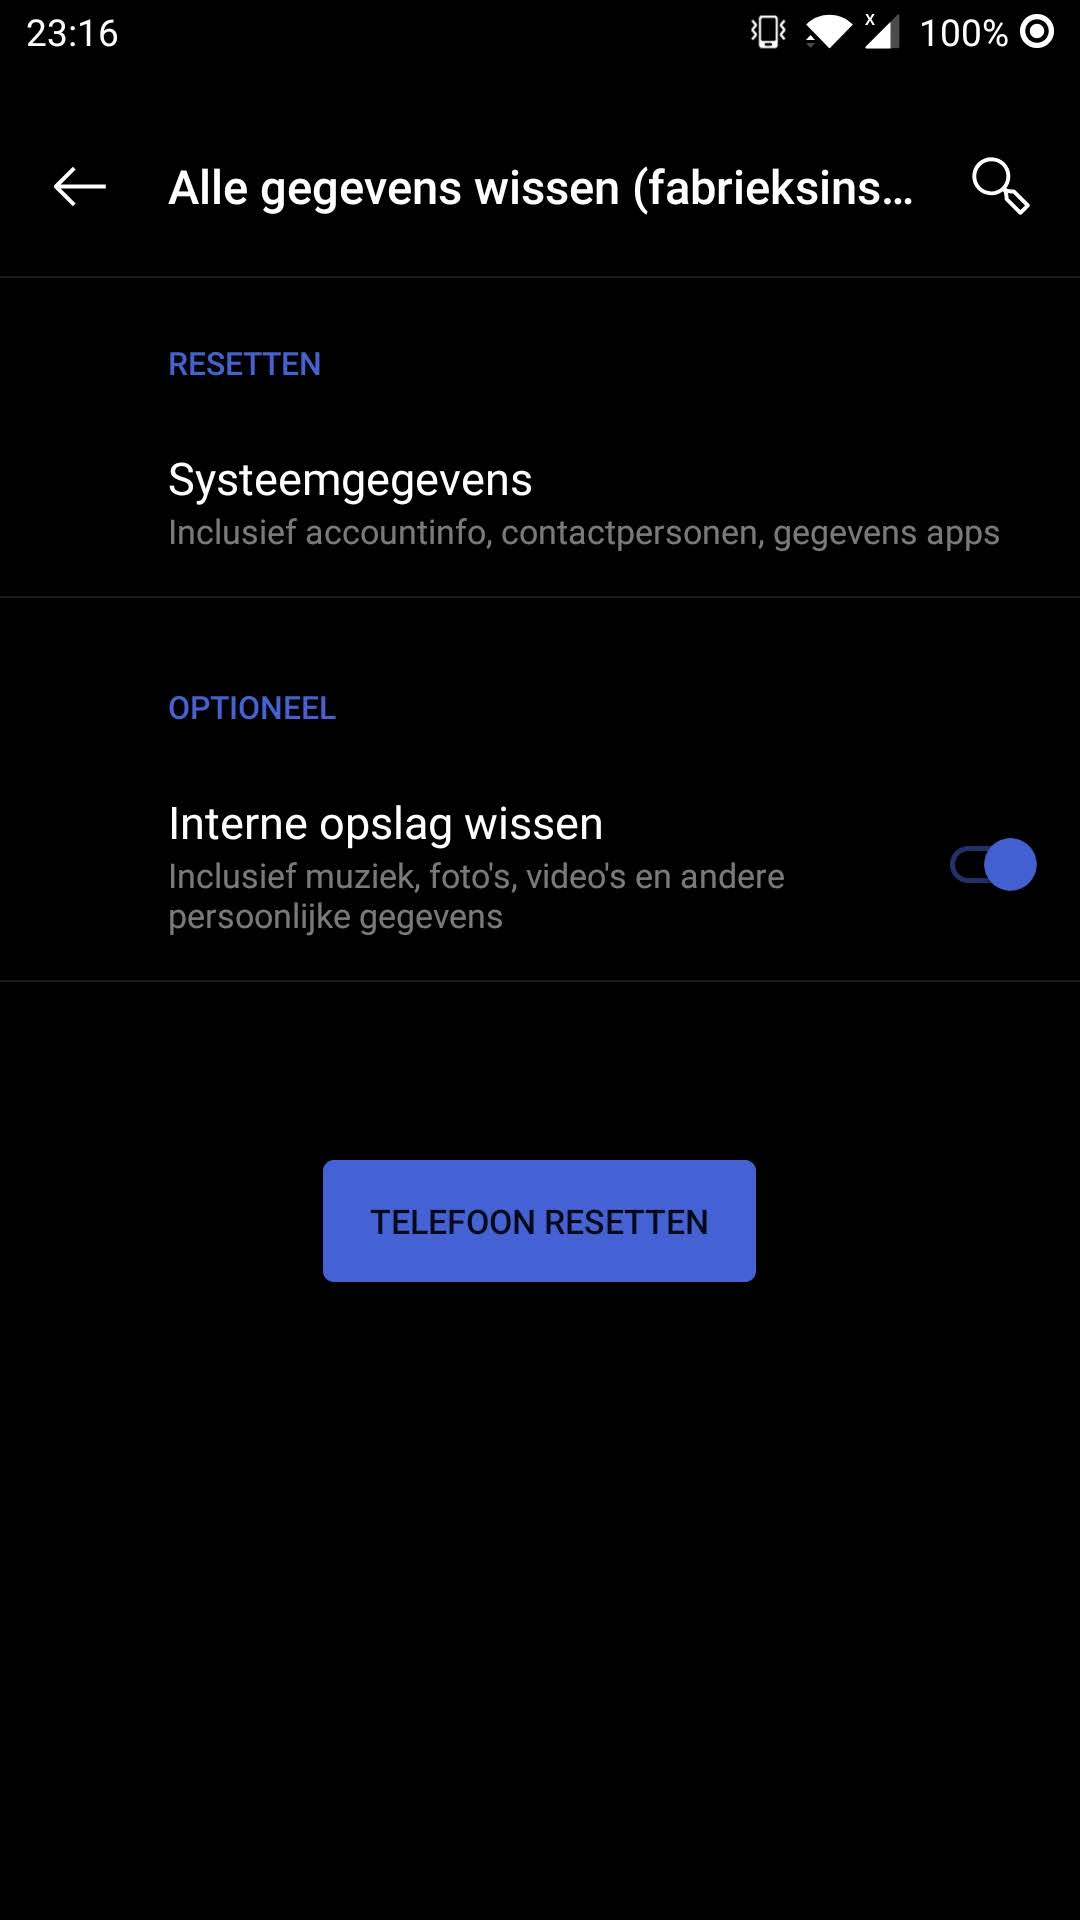
\includegraphics[width=0.4\textwidth]{img/fabrieksinstellingen.jpg}
    \caption{Screenshot van het scherm waar alle gegevens gewist kunnen worden en de fabrieksinstellingen kunnen worden teruggezet}
    \label{fig:fabrieksinstellingen}
\end{figure}


\subsection{Testgeval 2: Android met aangepaste instellingen}
\label{sec:testgeval2}
Binnen dit geval zal gebruik gemaakt worden van een Android apparaat waarbij de instellingen zo zijn aangepast dat de verzameling van data geminimaliseerd wordt. Dit zal gedaan worden via de 'zachte' methoden die besproken werden in het literatuuronderzoek (\ref{softmethods}), maar beperkt zich hier niet toe.

\subsection{Testgeval 3: Aangepaste versie van Android}
\label{sec:testgeval3}
Dit testgeval maakt gebruik van een Android apparaat waarop LineageOS is geïnstalleerd. LineageOS is een custom ROM (zie \ref{installcustomrom}) waarbij het 'Google Apps' pakket niet is inbegrepen in het besturingssysteem. Er zal gebruik gemaakt worden van de laatste officiële versie van LineageOS voor dit apparaat die microG reeds omvat, namelijk 16.0, die te vinden is op \url{https://download.lineage.microg.org/cheeseburger/} (de term 'cheeseburger' in de URL is de codenaam voor de 'Oneplus 5', het testapparaat). Deze ROM is een aangepaste versie van de officiële versie van LineageOS, die enkel kleine wijzigingen aanbracht om zo MicroG standaard mee te kunnen leveren.

\section{Methode voor monitoring netwerkactiviteit}
\label{sec:metingsoftware}
Het verzamelen van data die de netwerkactiviteit van het apparaat beschrijft, zal op een gelijkaardige manier worden gedaan zoals in het onderzoek door \cite{schmidt_google-data-collection}, wat ook in de literatuurstudie werd besproken. Om exact te kunnen zien welke data er precies binnenkomt en buitengaat via het internet op het apparaat, is er extra software nodig. Deze optie wordt namelijk niet gegeven door het Android besturingssysteem zelf. De software die wij gebruiken moet voldoen aan enkele voorwaarden:
\begin{itemize}
    \item De verkregen data moet kunnen worden geëxporteerd naar een bruikbaar formaat.
    \item De software mag geen aanpassing maken aan of vereisen van het apparaat.
    \item De software moet de gevraagde data verzamelen zonder dat deze wordt beïnvloed door de software zelf.
\end{itemize}
Er bestaan reeds veel applicaties die rechtstreeks vanaf het Android apparaat deze data kunnen verzamelen. Vele hiervan vallen al direct weg, aangezien ze root toegang vereisen. De 'geroote' toestand is namelijk een voorwaarde van de testgevallen, waardoor we deze doorheen de gevallen niet ingeschakeld kunnen houden. 

De uiteindelijke gekozen software is 'Charles Proxy'. Deze software is makkelijk in gebruik en kan de gedetailleerde resultaten van een monitoring sessie exporteren naar een '.csv' bestand, waar makkelijk mee gewerkt kan worden. De techniek die in dit programma wordt gehanteerd staat gekend als 'MITM', wat letterlijk 'Man-In-The-Middle' betekent. Zoals de naam al zegt is dit een proxy die als 'tussenpersoon' tussen het apparaat en het internet zal staan, en zo alle netwerkactiveit zal kunnen monitoren. Wanneer deze applicatie draait op een computer binnen een netwerk, moeten er op het Android apparaat nog twee extra instellingen gebeuren voordat al het netwerkverkeer kan worden opgevolgd. Eerst en vooral moet het Android apparaat verbonden zijn met hetzelfde netwerk als de computer waarop Charles draait. Daarna moet het netwerk op het Android apparaat zo worden ingesteld dat al het verkeer eerst via de proxy op de computer passeert. Hiervoor moet gekeken worden wat het lokale IP-adres is van deze computer binnen het netwerk. Op windows computers kan deze gevonden worden via het 'ipconfig' commando en op Mac computers via het 'ifconfig' commando. Eens gevonden moet dit IP-adres als proxy ingevoerd worden in de netwerkinstellingen binnen het Android apparaat. Dit kan gedaan worden door te navigeren naar de Wi-Fi instellingen, het verbonden netwerk te selecteren en dan op het potloodje te drukken om de instellingen van dit netwerk te wijzigen. Bij 'Hostnaam van proxy' moet dan het lokaal IP-adres van de computer worden ingegeven, en in het 'Proxy-Poort' veld 8888 (Dit is de standaard poort die Charles Proxy gebruikt). 

Zodra het Android apparaat een verbinding probeert te maken met een website zal Charles een melding tonen die vraagt of het apparaat dat probeert verbinding te maken wel degelijk toegang mag hebben tot de proxy, zoals te zien in figuur \ref{fig:charlesmelding}. Hier dient op 'allow' geklikt te worden. 

\begin{figure}
    \centering
    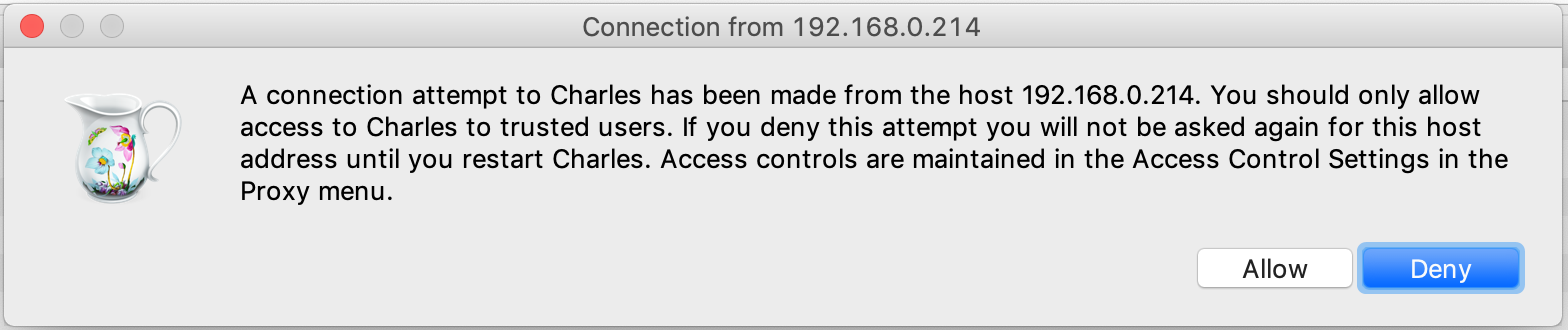
\includegraphics[width=1\textwidth]{img/charlesmelding.png}
    \caption{Screenshot van de melding die Charles geeft wanneer er een nieuwe onbekende verbinding binnenkomt}
    \label{fig:charlesmelding}
\end{figure}

Vanaf dit moment kan het Android apparaat verbinden met het internet, doorheen de proxy. Binnen dit onderzoek willen we voornamelijk te weten komen hoeveel data er nog naar Google wordt gecommuniceerd binnen de verschillende testgevallen. De inhoud en de specifieke URL van de aanvraag zijn hier dus minder van belang. Het decoderen van SSL aanvragen zou beteken dat er meer informatie kan worden verzameld over de inhoud en specifieke URL van de aanvraag, maar ook dat sommige aanvragen zouden falen. Applicaties zullen al dan niet reageren op mislukte aanvragen door deze gewoon opnieuw te proberen versturen. Dit zou dus een vertekend beeld geven van de realiteit. Daarom zal decodering van SSL aanvragen niet gebruikt worden in dit experiment. 

\subsection{Verdere analyse van gecodeerde verzoeken}
Deze methode zal binnen dit niet onderzoek niet worden toegepast, aangezien de extra verzamelde informatie het originele doel van het experiment te veel zou beïnvloeden. Deze sectie is dus louter informatief voor toekomstige onderzoeken die wel de inhoud en specifieke URL van de aanvraag zouden moeten analyseren.

Indien we de door een SSL-certificaat versleutelde informatie wel zouden willen onderscheppen, zou binnen Charles in de 'SSL Proxying Settings' ingesteld moeten worden dat SSL verzoeken ook door de proxy zullen gaan. Bij deze instelling kan dan per domein ingesteld worden of SSL verzoeken onderschept worden of niet ('*:*' zal dit voor alle domeinen en alle poorten doen). Zo kan ook van deze aanvragen de inhoud in vlakke tekst bekeken worden, samen met de exacte URL van de aanvraag. 

Wanneer er nu naar een site wordt gesurft op het Android apparaat zal er nog steeds een melding worden weergegeven die zegt dat de verbinding onveilig is, zoals te zien in figuur \ref{fig:charlescantconnect}. Dit komt doordat Charles gebruik maakt van zijn eigen SSL certificaat, dat nog niet als een vertrouwd certificaat wordt beschouwd binnen het Android apparaat.

\begin{figure}
    \centering
    \begin{subfigure}{.5\textwidth}
        \centering
        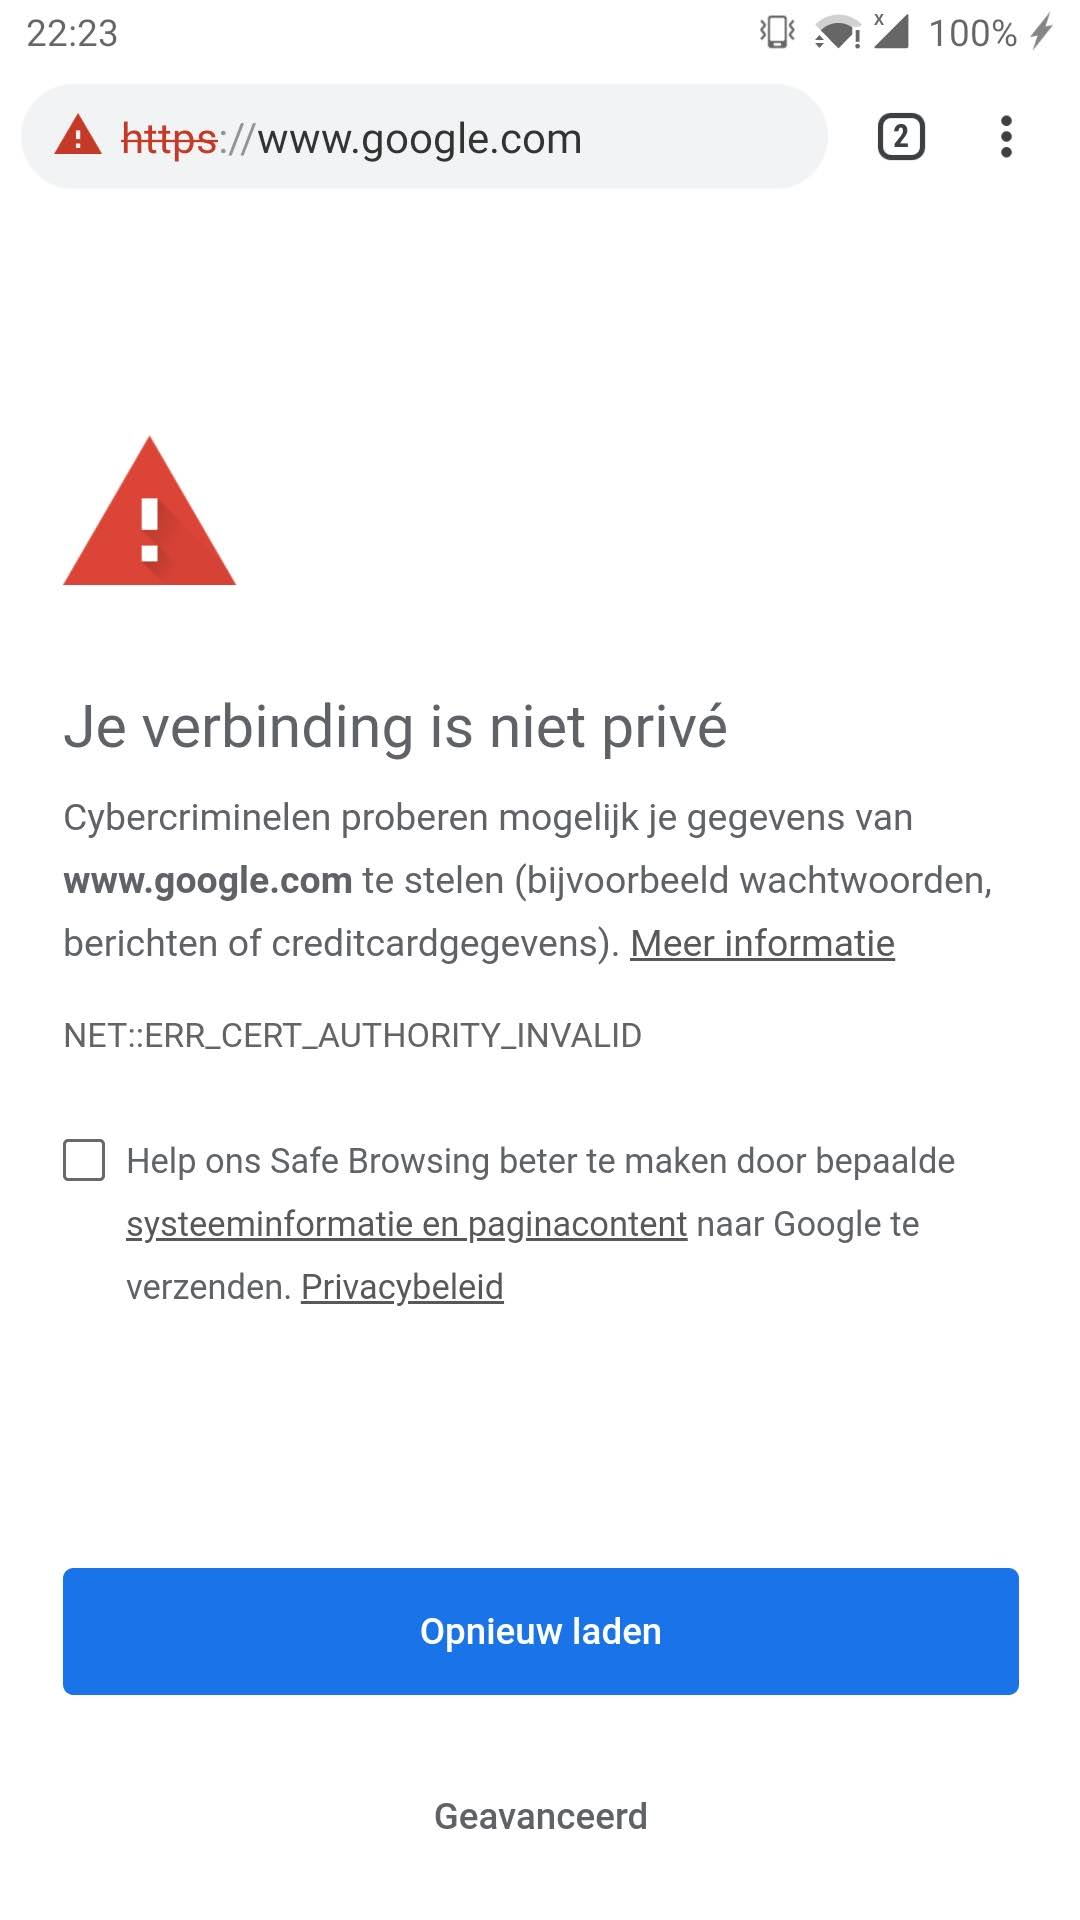
\includegraphics[width=0.8\linewidth]{img/charlescantconnect.jpg}
        \caption{Sites kunnen niet bereikt worden door een onveilig certificaat}
        \label{fig:charlescantconnect}
    \end{subfigure}%
    \begin{subfigure}{.5\textwidth}
        \centering
        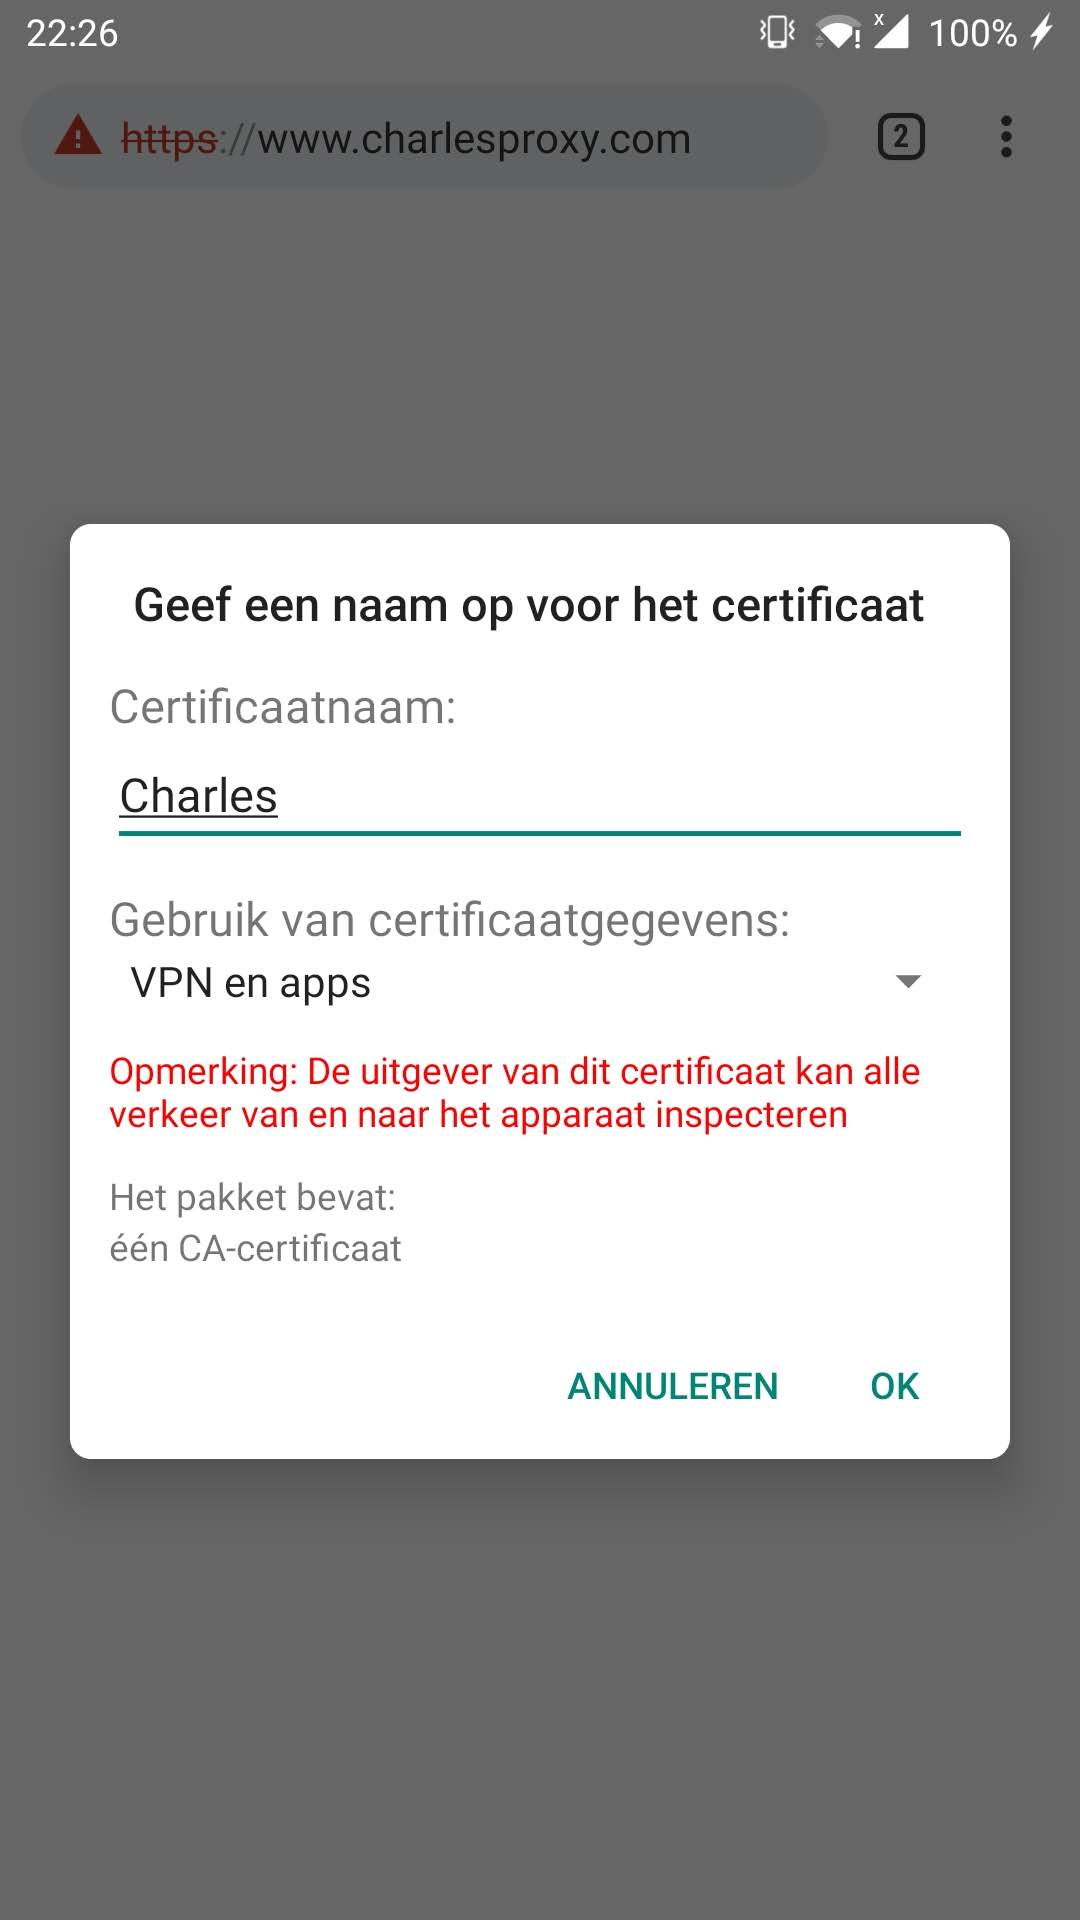
\includegraphics[width=0.8\linewidth]{img/charlessslcertificateinstall.jpg}
        \caption{Installatie van het gedownloade Charles SSL certificaat}
        \label{fig:charlessslcertificateinstall}
    \end{subfigure}
    \caption{Het Charles SSL certificaat downloaden en gebruiken}
\end{figure}

Door op het apparaat naar \url{http://www.charlesproxy.com/getssl/} (de enige pagina die browser wel zal kunnen bereiken wanneer SSL proxying is ingeschakeld) te surfen, wordt het Charles certificaat gedownload, en kan dit geïnstalleerd worden op het apparaat, zoals te zien in figuur \ref{fig:charlessslcertificateinstall}.

Sommige applicaties gebruiken echter een systeem genaamd 'SSL Certificate Pinning'.  Apps die ontwikkeld zijn met Android Marshmallow (6.0) of lager als doelversie, zullen automatisch certificaten aanvaarden die door gebruikers geïnstalleerd zijn. Van zodra de applicatie gericht is op een hogere versie van Android, heeft de ontwikkelaar de mogelijkheid om 'SSL Certificate Pinning' toe te passen. Op lagere versies van Android was dit ook mogelijk, maar moest dit volledig door de ontwikkelaar zelf worden geïmplementeerd, waardoor dit vaak niet gebeurde. Hetgeen wat nieuw is in Android Nougat (7.0) is dat dit extreem makkelijk is geworden door de introducite van 'Network Security Configuration'. SSL Certificate Pinning houdt in dat de ontwikkelaar, indien hij/zij dit wil, kan afdwingen dat er een bepaald certificaat wordt gebruikt wanneer er met zijn/haar server gecommuniceerd wordt  \autocite{wass_ssl-pinning}. Het Charles certificaat zal hier dan worden geweigerd, en de aanvraag zal falen.

Om te zorgen dat dit verkeer wel wordt doorgelaten, zou het  afgedwongen certificaat moeten gewijzigd worden. Deze ligt echter vastgelegd binnen de code van de applicatie. Er bestaan wel tools zoals het 'Frida framework' die tijdens het uitvoeren van een bepaalde applicatie het afgedwongen certificaat kunnen wijzigen door middel van code injectie. Deze methoden vereisen echter root en zijn gelimiteerd tot opstartbare applicaties. Applicaties zoals Google Play-services hebben geen grafische gebruikersinterface, en kunnen op deze manier niet omzeild worden. Een andere mogelijk is het manueel aanpassen van de programmatie van de applicatie. Hiervoor zou de applicatie die aangepast moet worden eerst gedecompileerd worden, de code ervan worden aangepast zodat ons certificaat wel wordt geaccepteerd, en dan worden hercompileerd naar een uitvoerbare applicatie. 

\section{Verloop experiment}
\label{sec:conditionsexperiment}
Binnen deze sectie zal worden besproken hoe het experiment precies zal verlopen en welke voorwaarden van toepassing zijn.

\subsection{Uitschrijven stappenplan per testgeval}
Per testgeval zal een stappenplan worden uitschreven dat in detail vermeldt hoe de toestand van het testgeval bereikt wordt. Indien hier moeilijkheden bij optreden, dienen die ook opgenomen te worden. Terugkerende stappen kunnen eventueel vooraf gedefinieerd worden, en naar worden verwezen vanuit het stappenplan van een testgeval.

\subsection{Meten van verzamelde data}
Bij alle testgevallen zullen Wi-Fi, bluetooth, en locatie ingeschakeld zijn. Dit wordt gedaan zodat er op elk moment genoeg data is die mogelijk naar Google kan worden verzonden. Wanneer de hoeveelheid van mogelijk te verzamelen data groter is, zorgt dit ook voor preciezere metingen van de werkelijk doorgestuurde data. Ook  testen we tot op welke mate we dataverzameling kunnen beperken zonder functionaliteit te beperken. Wanneer we voorgenoemde verbindingsmethoden uitschakelen, wordt de functionaliteit van het apparaat beperkt. Het testapparaat zal via een 5 GHz Wi-Fi verbinding verbonden zijn met een beveiligd Wi-Fi netwerk. Mobiele data zal uitgeschakeld blijven, aangezien we via de gebruikte software hiervan de netwerkactiviteit niet kunnen monitoren.

Gedurende één uur zal de netwerkactiviteit van het apparaat gemonitord worden. Tijdens deze tijd zal het apparaat stilliggen en zal er ook geen interactie met het apparaat gebeuren. Het apparaat zal ook zodanig ingesteld zijn dat deze niet in slaapmodus valt, wat mogelijk de resultaten kan beïnvloeden. Er wordt niet gebruik gemaakt van modussen die de batterijduur zouden verlengen, en het apparaat zal tijdens het experiment aangesloten zijn aan zijn oplader. Voor elk testgeval zal een nieuw Google account gebruikt worden, indien vereist. Dit experiment kan meerdere keren uitgevoerd worden voor een betere benadering van realistische data.





%%=============================================================================
%% Resultaten
%%=============================================================================

\chapter{Resultaten}
\label{ch:resultaten}

\section{Stappenplannen testgevallen}

\subsection{Terugkerende stappen}
\label{recurringsteps}

Hier worden stappen gedefiniëerd die doorheen de testgevallen gebruikt worden.

\begin{enumerate}
    \item 
    \label{factoryreset}
    Het apparaat moet worden teruggezet naar de fabrieksinstellingen, en alle data moet worden gewist. Dit kan gedaan worden door binnen de instellingen applicatie te navigeren naar 'Systeem' > 'Opties voor resetten' > 'Alle gegevens wissen (fabrieksinstellingen terugzetten)'. Hier moet 'interne opslag wissen' aangeduid worden, voordat er op 'telefoon resetten' wordt gedrukt, zoals te zien in figuur \ref{fig:fabrieksinstellingen}. Bevestig deze actie door de pincode van het apparaat in te vullen, indien deze is ingesteld. Druk hierna op 'Alles wissen'. De telefoon wordt nu gereset en heropgestart.
    \item 
    \label{initialsetup}
    Wanneer de telefoon teruggezet is naar de fabrieksinstellingen, zal er gevraagd worden om de initïele setup opnieuw te voltooien. Hier moet telkens de standaard optie aangeduid worden, behalve als er hier wordt vermeld een andere optie te nemen.
    \begin{itemize}
        \item Apps en gegevens kopiëren: druk op 'gegevens niet kopiëren'. We willen hier met een 'vers' Android besturingssysteem werken.
        \item Inloggen met Google: Kies hier om een nieuw account aan te maken.
        \item Gezichtsontgrendeling: Dit heeft geen belang voor dit experiment, en mag overgeslaan worden.
        \item Vingerafdruk ontgrendeling: Dit heeft geen belang voor dit experiment, en mag overgeslaan worden.
        \item Google Pay: Dit heeft geen belang voor dit experiment, en mag overgeslaan worden.
    \end{itemize}
    \item 
    \label{setupgoogleapps}
    Stel de Google applicaties in. Ga één voor één door de applicaties in figuur \ref{fig:googleapps} en doorloop  het initële setup proces. Wanneer er gevraagd wordt om machtigingen te verlenen aan de applicatie, druk dan op toestaan. Open ook de Google Play Store, ga naar 'Mijn apps en games' en druk op 'Alles updaten'.
    \item 
    \label{developersettings}
    We moeten in de ontwikkelaarsopties van het apparaat een instelling aanpassen. Standaard zijn deze instellingen niet zichtbaar. Om deze in te schakelen drukt navigeert u naar 'Instellingen' > 'Over de telefoon'. Druk 7 keer na elkaar op de sectie 'Build-nummer'. Er komt een melding op het scherm die zegt dat we nu een ontwikkelaar zijn. De ontwikkelaarsopties zijn te bereiken op 'Instellingen' > 'Systeem' > 'Ontwikkelaarsopties'
    \item 
    \label{disablesleep}
    Er moet ingesteld worden dat het scherm niet uitvalt terwijl het experiment loopt. Navigeer naar 'Instellingen' > 'Systeem'. Onderaan is er nu een nieuwe optie verschenen die 'Ontwikkelaarsopties' noemt. Druk hierop en zoek naar de instelling 'Stand-by'. Door deze aan te zetten zal het scherm van het apparaat niet meer uitvallen wanneer deze aan stroom is aangesloten.
\end{enumerate}

\begin{figure}
    \centering
    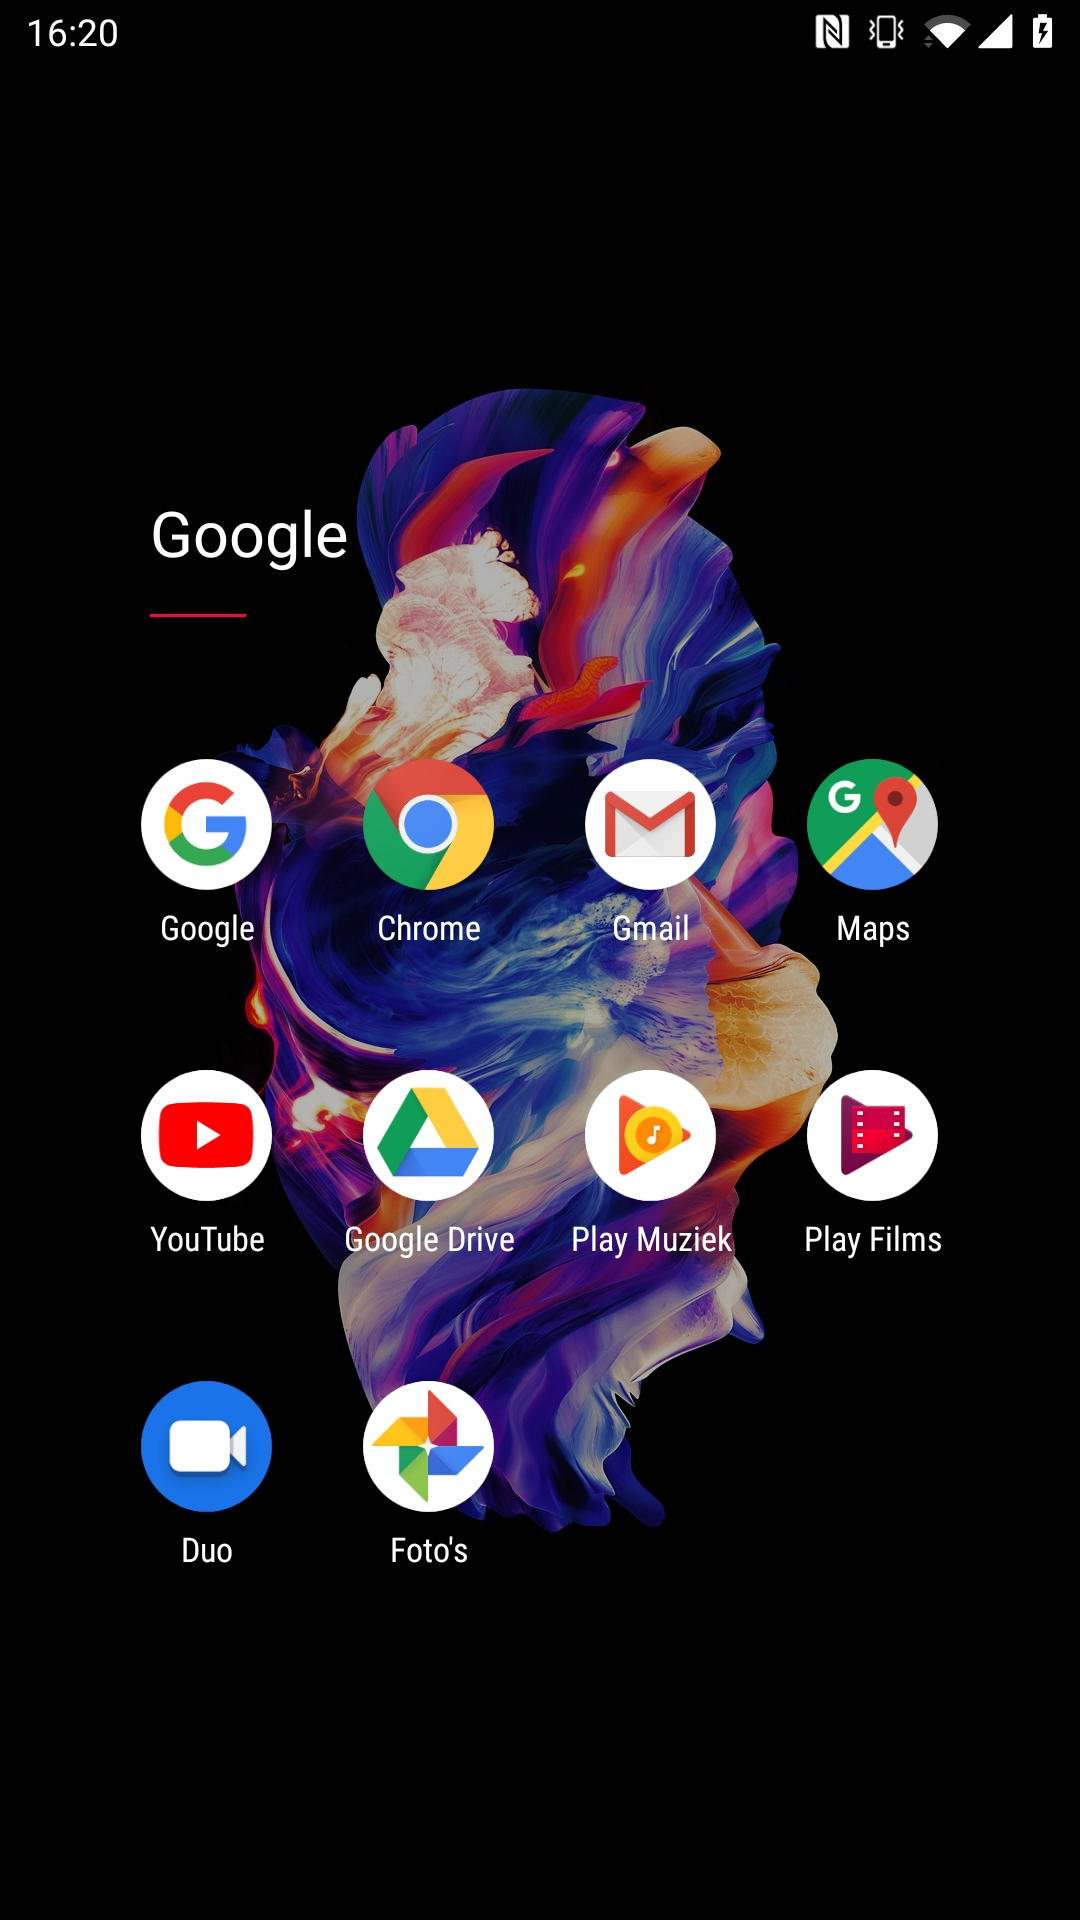
\includegraphics[width=0.4\textwidth]{img/googleapps.jpg}
    \caption{Screenshot van de google applicaties die moeten worden geopend en ingesteld}
    \label{fig:googleapps}
\end{figure}

\subsection{Testgeval 1: Android met fabrieksinstellingen}

Voor de toestand van dit testgeval te bekomen, moeten volgende stappen uitgevoerd worden.
\begin{enumerate}
    \item Stap \ref{factoryreset} van terugkerende stappen (\ref{recurringsteps})
    \item Stap \ref{initialsetup} van terugkerende stappen (\ref{recurringsteps})
    \item Stap \ref{setupgoogleapps} van terugkerende stappen (\ref{recurringsteps})
    \item Stap \ref{developersettings} van terugkerende stappen (\ref{recurringsteps})
    \item Stap \ref{disablesleep} van terugkerende stappen (\ref{recurringsteps})
\end{enumerate}


\subsection{Testgeval 2: Android met aangepaste instellingen}

Voor de toestand van dit testgeval te bekomen, moeten volgende stappen uitgevoerd worden.

\begin{enumerate}
    \item Stap \ref{factoryreset} van terugkerende stappen (\ref{recurringsteps})
    \item Stap \ref{initialsetup} van terugkerende stappen (\ref{recurringsteps})
    \item Schakel persoonlijke advertenties uit. Navigeer hievoor naar 'Instellingen' > 'Google' > 'Advertenties'. Zet hier 'Afmelden voor personalisatie van advertenties' aan.
    \item Stop de data verzameling van locatiegegevens. Dit kan via de webapplicatie van Google gedaan worden of via het apparaat zelf. Voor dit te doen via het apparaat zelf, dient men eerst te navigeren naar 'Instellingen' > 'Google' > 'Google account'. Ga dan naar het tabblad 'Gegevens en personalisatie'. Onder de sectie 'Activiteitsopties' moeten 'Web- en app-activiteit' en 'Locatiegeschiedenis' onderbroken worden.
    \item Stel een andere DNS-server in. Navigeer hiervoor naar 'Instellingen' > 'Wi-Fi \& internet' > 'Privé-DNS'. Hier kan de gebruiker een DNS-provider naar keuze invullen. Voor dit experiment zal de '1dot1dot1dot1.cloudflare-dns.com' gebruikt worden, een DNS-provider aangeboden door cloudflare.
    \item Stap \ref{disablesleep} van terugkerende stappen (\ref{recurringsteps})
    \item Stop met het gebruiken van Google applicaties. Hiervoor hoeft er in principe geen extra stap worden uitgevoerd, maar er kan wel gezorgd worden dat reeds geïnstalleerde Google applicaties niet meer kunnen worden uitgevoerd op de achtergrond. Voor dit experiment zullen de volgende applicaties uitgeschakeld worden: Google Agenda, Google Chrome, Google Contacten, Google Drive, Google Duo, Google Foto's, GBoard, Gmail, Google, Google Play Films, Google Play Muziek, Google Play Store, Google Maps, Youtube. Om dit te doen moet men eerst navigeren naar 'Instellingen' > 'Apps en meldingen' > 'Alle 40 apps bekijken'. Druk één voor één de applicatie aan die u wilt uitschakelen, en druk in het detailscherm op 'uitschakelen'.
\end{enumerate}
    
\subsection{Testgeval 3: Aangepaste versie van Android}

Voor de toestand van dit testgeval te bekomen, moeten volgende stappen uitgevoerd worden.

\begin{enumerate}
    \item Installeer ADB, Fasboot en Android drivers op een computer. Deze tools geven ons de mogelijkheid om commando's te versturen vanaf onze computer naar de bootloader of herstelmodus van ons apparaat. Een gids voor het installeren van deze tools op verschillende platforms is te vinden op \url{https://www.xda-developers.com/install-adb-windows-macos-linux/}.
    \item Stap \ref{setupgoogleapps} van terugkerende stappen (\ref{recurringsteps})
    \item Schakel USB-foutopspring in. Deze optie moet ingeschakeld worden zodat een computer kan communiceren met het apparaat via een USB-kabel.
    \item Ontgrendel de bootloader van het apparaat. Dit is nodig voor een custom ROM te kunnen installeren op het apparaat. Om dit te doen met OEM-ontgrendeling worden ingeschakeld. Deze optie bevindt zich in 'Instellingen' > 'Systeem' > 'Ontwikkelaarsopties'. Schakel ook 'Geavanceerd herstarten' in. Deze optie laat ons het apparaat makkelijk heropstarten naar de herstelmodus en de bootloader van ons apparaat. Houdt de aan-knop van het apparaat lang in tot er aan de rechterzijde van het scherm opties tevoorschijn duiken. Druk hier op 'Bootloader'. Sluit het apparaat aan op de computer met een USB-kabel, en open een terminal venster. Typ hierin 'fastboot oem unlock' en druk op enter. Op het apparaat verschijnt nu een keuzemenu. Selecteer door middel van de volumeknoppen 'Unlock the booatloader' en bevestig met de aan-knop het apparaat. De bootloader is nu ontgrendeld.
    \item 
    Installeer een custom recovery. Deze hebben we nodig om een custom ROM te kunnen installeren. Eerst moeten we hiervoor het '.img' bestand hiervan downloaden. TWRP is de meest gekende custom recovery, aangezien deze heel wat handige functies aanbiedt. Voor dit experiment wordt er gebruik gemaakt van een aangepaste versie heirvan, namelijk TWRP blu\_spark, wegens compatibiliteitsproblemen met het testapparaat. Deze is te vinden op \url{https://github.com/engstk/android_device_oneplus_cheeseburger/releases}. Navigeer in het terminal venster naar de locatie waar dit bestand opgeslagen is, en typ 'fastboot flash recovery lineage-16.0-20190513-microG-cheeseburger.zip'. Hierna kunnen we via de volumeknoppen navigeren naar 'Recovery mode' en deze selecteren door middel van de aan-knop.
    \item Nu moet het ROM bestand overgezet worden naar het apparaat. Navigeer naar de locatie waar het ROM bestand zich bevindt en typ 'adb push lineage-16.0-20190513-microG-cheeseburger.zip /data/tmp/lineage.zip'. Het bestand wordt nu overgezet naar het apparaat.
    \item Wis het apparaat door binnen TWRP op 'Wipe' te drukken. Selecteer 'Advanced wipe' en klik 'System', 'Data' en 'Cache' aan en bevestig.
    \item Installeer de ROM. Druk binnen TWRP op 'Install' en navigeer naar '/data/tmp/'. Selecteer lineage.zip en bevestig de installatie van dit .zip bestand. Eens de installatie voltooid is druk je op 'Wipe cache/dalvik', en daarna op 'Reboot System'.
    \item 
    LineageOS is nu geïnstalleerd! Merk op dat er op het apparaat geen Google applicaties te vinden zijn. De aanwezigheid van microG zorgt ervoor dat applicaties die normaal voortwerken op API's die Google Play-services aanbieden, nog steeds werken.
    \item Stap \ref{disablesleep} van terugkerende stappen
\end{enumerate}

\section{Monitoring netwerkactiviteit}

\subsection{Testgeval 1: Android met fabrieksinstellingen}

\subsection{Testgeval 2: Android met aangepaste instellingen}

\subsection{Testgeval 3: Aangepaste versie van Android}

% Voeg hier je eigen hoofdstukken toe die de ``corpus'' van je bachelorproef
% vormen. De structuur en titels hangen af van je eigen onderzoek. Je kan bv.
% elke fase in je onderzoek in een apart hoofdstuk bespreken.

%\input{...}
%\input{...}
%...

%%=============================================================================
%% Conclusie
%%=============================================================================

\chapter{Conclusie}
\label{ch:conclusie}

% TODO: Trek een duidelijke conclusie, in de vorm van een antwoord op de
% onderzoeksvra(a)g(en). Wat was jouw bijdrage aan het onderzoeksdomein en
% hoe biedt dit meerwaarde aan het vakgebied/doelgroep? 
% Reflecteer kritisch over het resultaat. In Engelse teksten wordt deze sectie
% ``Discussion'' genoemd. Had je deze uitkomst verwacht? Zijn er zaken die nog
% niet duidelijk zijn?
% Heeft het onderzoek geleid tot nieuwe vragen die uitnodigen tot verder 
%onderzoek?

%%\lipsum[76-80]



%%=============================================================================
%% Bijlagen
%%=============================================================================

\appendix
\renewcommand{\chaptername}{Appendix}

%%---------- Onderzoeksvoorstel -----------------------------------------------

\chapter{Onderzoeksvoorstel}

Het onderwerp van deze bachelorproef is gebaseerd op een onderzoeksvoorstel dat vooraf werd beoordeeld door de promotor. Dat voorstel is opgenomen in deze bijlage.

% Verwijzing naar het bestand met de inhoud van het onderzoeksvoorstel
%---------- Inleiding ---------------------------------------------------------

\section{Introductie} % The \section*{} command stops section numbering
\label{sec:introductie}

%Hier introduceer je werk. Je hoeft hier nog niet te technisch te gaan.

%Je beschrijft zeker:

%\begin{itemize}
%  \item de probleemstelling en context
%  \item de motivatie en relevantie voor het onderzoek
%  \item de doelstelling en onderzoeksvraag/-vragen
%\end{itemize}
Het is reeds zeer actueel dat er heel veel persoonlijke data wordt bijgehouden bij het gebruiken van online services. Het probleem ligt dan ook bij het feit dat de gebruikers van deze services niet voldoende weten waarom deze data wordt bijgehouden, wat er mee gedaan wordt en waarom ze dit misschien beter zouden voorkomen. Denk in dit verband ook aan de GDPR-wetgeving die eveneens werd ingevoerd in functie van het beter informeren van de Europese burger over welke data er over hem/haar wordt opgeslagen. 

\vspace{3mm}

\noindent In mijn werk zal dieper worden ingegaan op wat er precies wordt bijgehouden van data bij het gebruik van het Android besturingssysteem, waarom dit gebeurt, en hoe het vermeden kan worden. Dit kadert in de bescherming van de persoonlijke levenssfeer. 

\vspace{3mm}

\noindent De onderzoeksvragen voor mijn werk zijn dan als volgt:


\begin{itemize}
	\item Welke data wordt er bij het gebruik van het Android besturingssysteem exact bijgehouden door Google?
	\item Welke opties worden reeds door Google aangeboden om het delen van deze data te beperken?
	\item Kan Google volledig verbannen worden uit het Android besturingssysteem, en hoe?
	\item Zijn er voldoende alternatieven om de functionaliteiten die Google biedt te vervangen, en welke zijn deze?
	\item Zijn Android gebruikers voldoende ingelicht over de hoeveelheid data dat ze delen met Google?
\end{itemize}


%---------- Stand van zaken ---------------------------------------------------

\section{Stand van zaken}
\label{sec:state-of-the-art}

%Hier beschrijf je de \emph{state-of-the-art} rondom je gekozen onderzoeksdomein. Dit kan bijvoorbeeld een literatuurstudie zijn. Je mag de titel van deze sectie ook aanpassen (literatuurstudie, stand van zaken, enz.). Zijn er al gelijkaardige onderzoeken gevoerd? Wat concluderen ze? Wat is het verschil met jouw onderzoek? Wat is de relevantie met jouw onderzoek?
Aangezien Android eigendom is van Google, is het ook vanzelfsprekend dat Google heeft gezorgd dat de Google services zeer nauw geïntegreerd zijn in, zelfs verweven, in het smartphone besturingssysteem Android. Deze nauwe integratie heeft hierdoor dan ook als nadeel dat Google toegang heeft tot alle informatie over wat je via deze services doet.

\vspace{3mm}

\noindent Over dit onderwerp werden reeds verschillende artikels geschreven vanuit diverse invalshoeken. Dit gaat dan over artikelen die enkel beschrijven hoe Android zonder Google verwezenlijkt kan worden, zoals het artikel door \autocite{BertelKing2016}. Andere artikelen focussen dan meer op de alternatieven die kunnen gebruikt worden in plaats van Google applicaties, zoals het artikel door \autocite{EricFerrari2017}. Geen enkele van de artikelen zijn wetenschappelijk opgesteld, evenwel geven ze geen totaalbeeld van de problematiek. Mijn doelstelling is om deze problematiek zelf op een systematische en gestructureerde manier te onderzoeken.

%Verwijs bij elke introductie van een term of bewering over het domein naar de vakliteratuur, bijvoorbeeld~\autocite{Doll1954}! Denk zeker goed na welke werken je refereert en waarom.

% Voor literatuurverwijzingen zijn er twee belangrijke commando's:
% \autocite{KEY} => (Auteur, jaartal) Gebruik dit als de naam van de auteur
%   geen onderdeel is van de zin.
% \textcite{KEY} => Auteur (jaartal)  Gebruik dit als de auteursnaam wel een
%   functie heeft in de zin (bv. ``Uit onderzoek door Doll & Hill (1954) bleek
%   ...'')

%Je mag gerust gebruik maken van subsecties in dit onderdeel.

%---------- Methodologie ------------------------------------------------------
\section{Methodologie}
\label{sec:methodologie}

%Hier beschrijf je hoe je van plan bent het onderzoek te voeren. Welke onderzoekstechniek ga je toepassen om elk van je onderzoeksvragen te beantwoorden? Gebruik je hiervoor experimenten, vragenlijsten, simulaties? Je beschrijft ook al welke tools je denkt hiervoor te gebruiken of te ontwikkelen.

\subsection{{Kwalitatief en experimenteel onderzoek}}


Eerst en vooral zal bekeken worden welke data er allemaal wordt bijgehouden bij het gebruik van een Android telefoon.

\vspace{3mm}

\noindent Vervolgens zal worden nagegaan welke opties om het delen van data te beperken ons worden aangeboden vanuit het besturingssysteem zelf. Hier gaat het nog niet over het 'verbannen' van Google. Of dit beperkingen zou leggen op bepaalde functionaliteiten van Android wordt natuurlijk ook onderzocht.

\vspace{3mm}

\noindent Daarna zal het bestudeer worden of het mogelijk is Google volledig te verbannen uit de wortels van het Android besturingssysteem, door middel van methodes die niet direct door Android en Google zelf worden ondersteund.

\vspace{3mm}

\noindent Wanneer je niet meer met Google services werkt, betekent dit uiteraard dat je veel functionaliteit zal mislopen, aangezien dit niet het beoogde gebruik is volgens Google. Er zal onderzocht worden hoe deze verloren functionaliteiten zoveel mogelijk terug ingevuld kunnen worden door alternatieven, en in welke mate deze alternatieven opwegen tegen de standaard implementatie.

\vspace{3mm}

\noindent Aangezien reeds veel van deze informatie beschikbaar is op het internet, zullen voorgenoemde onderzoeken voornamelijk gebeuren via opzoekwerk en verificatie of deze informatie ook klopt, door middel van eigen experimenten.

\subsection{{Enquête}}

\noindent Naast deze onderzoeken kan er mogelijks ook een enquête uitgevoerd worden waarbij Android gebruikers worden gevraagd in welke mate ze op de hoogte zijn welke data ze reeds met Google delen door het gebruiken van hun Android telefoon.

%---------- Verwachte resultaten ----------------------------------------------
\section{Verwachte resultaten}
\label{sec:verwachte_resultaten}

%Hier beschrijf je welke resultaten je verwacht. Als je metingen en simulaties uitvoert, kan je hier al mock-ups maken van de grafieken samen met de verwachte conclusies. Benoem zeker al je assen en de stukken van de grafiek die je gaat gebruiken. Dit zorgt ervoor dat je concreet weet hoe je je data gaat moeten structureren.
Ik verwacht dat Google een zeer grote hoeveelheid gebruiksdata zal bijhouden per gebruiker. Dit zou dan gaan over alles wat je doet via Google services, zoals locatiegegevens, items die je hebt opgezocht, welke apps je allemaal staan hebt, etc.

\vspace{3mm}

\noindent Bij de vraag of Google zelf al mogelijkheden biedt om het delen van data te beperken kan men ervan uitgaan dat Google in Android zelf al heel wat mogelijkheden geeft om dit te doen. Naar mijn verwachtingen toe zullen deze opties de gebruiker echter nog steeds niet genoeg controle geven. Google zal hiernaast tevens nog steeds over een zeer grote hoeveelheid data van deze gebruiker blijven beschikken.

\vspace{3mm}

\noindent Aangezien de Android development community reeds zeer groot is,is het zeer goed mogelijk is dat er reeds manieren ontwikkeld zijn om Google volledig te verbannen uit Android. Als dit mogelijk is, zullen er volgens mij zeker ook methodes bestaan om alle functionaliteiten die we verliezen door dit te doen, te vervangen door alternatieven. Deze alternatieven zullen waarschijnlijk niet even gestroomlijnd zijn als het aanbod van Google. 

\vspace{3mm}

\noindent Wat betreft mijn laatste onderzoeksvraag, zou men uit de verwachte resultaten kunnen concluderen dat mensen niet voldoende ingelicht zijn over de hoeveelheid data die ze met Google delen. Ik ga hiervan uit aangezien ik mezelf bestempel als een Android 'power user', en ikzelf eerder ook niet wist wat er juist werd bijgehouden.


%---------- Verwachte conclusies ----------------------------------------------
\section{Verwachte conclusies}
\label{sec:verwachte_conclusies}

%Hier beschrijf je wat je verwacht uit je onderzoek, met de motivatie waarom. Het is \textbf{niet} erg indien uit je onderzoek andere resultaten en conclusies vloeien dan dat je hier beschrijft: het is dan juist interessant om te onderzoeken waarom jouw hypothesen niet overeenkomen met de resultaten.

Uit de verwachte resultaten zou kan geconcludeerd worden dat Google een heel stuk meer gebruiksinformatie ter beschikking krijgt via haar smartphone besturingssysteem Android, dan dat mensen initieel zouden denken. De gebruikers van dit besturingssysteem zijn hiervan onvoldoende op de hoogte en zien bijgevolg hiervan ook de ernst niet in.

\vspace{3mm}

\noindent Een goed begin om de macht van Google op dit vlak wat in te perken zullen de opties zijn die Android ons zelf al aanbiedt. Dit zullen waarschijnlijk niet veel opties zijn, maar alles telt natuurlijk. 

\vspace{3mm}

\noindent Om nog verder te gaan zullen er manieren zijn om het besturingssysteem te modificeren zodat Google volledig verbannen wordt uit het besturingssysteem. Deze manieren zijn grotendeels afkomstig van Android gebruikers van de development community, die eveneens niet akkoord zijn met de hoeveelheid data die Android ophaalt en doorstuurt.


%TODO: Dependency op google services, ecosysteem?


%%---------- Andere bijlagen --------------------------------------------------
% Voeg hier eventuele andere bijlagen toe
%\input{...}

\chapter{Ruwe testresultaten}
\label{appendix:rawresults}

In dit hoofdstuk zullen de ruwe testresultaten die voortkkomen uit de monitoring van de netwerkactiviteit, zich bevinden. De velden die niet van belang waren voor dit onderzoek, zijn weggelaten. Weggelaten velden zijn 'Status', 'Protocol', 'Method', 'Content-Type', 'Client Address', 'Client Port', 'Remote Address', 'Remote Port', 'Exception', 'Request End Time', 'Response Start Time', 'Response End Time', 'Duration (ms)', 'DNS Duration (ms)', 'Connect Duration (ms)', 'SSL Duration (ms)', 'Request Duration (ms)', 'Response Duration (ms)', 'Latency (ms)', 'Speed (KB/s)', 'Request Speed (KB/s)', 'Response Speed (KB/s)', 'Request Handshake Size (bytes)', 'Request Header Size (bytes)', 'Request Body Size (bytes)', 'Response Handshake Size (bytes)', 'Response Header Size (bytes)', 'Response Body Size (bytes)', 'Request Compression' en 'Response Compression'. Verder is deze data onaangepast.

\section{Testgeval 1}

% Please add the following required packages to your document preamble:
% \usepackage{booktabs}
% \usepackage{longtable}
% Note: It may be necessary to compile the document several times to get a multi-page table to line up properly
\begin{longtable}[c]{@{}llll@{}}
    \toprule
    Request Start Time & URL & Response Code & Protocol \\* \midrule
    \endhead
    %
    \bottomrule
    \endfoot
    %
    \endlastfoot
    %
    29-05-19 15:05 & https://www.gstatic.com & 200 & https \\
    29-05-19 15:05 & https://www.gstatic.com & 200 & https \\
    29-05-19 15:05 & https://play.googleapis.com & 200 & https \\
    29-05-19 15:06 & https://www.gstatic.com & 200 & https \\
    29-05-19 15:06 & https://www.gstatic.com & 200 & https \\
    29-05-19 15:09 & https://update.googleapis.com & 200 & https \\
    29-05-19 15:12 & https://www.google.com & 200 & https \\
    29-05-19 15:12 & https://geomobileservices-pa.googleapis.com & 200 & https \\
    29-05-19 15:15 & https://android.googleapis.com & 200 & https \\
    29-05-19 15:15 & https://history.google.com & 200 & https \\
    29-05-19 15:15 & https://www.googleapis.com & 200 & https \\
    29-05-19 15:16 & https://play.googleapis.com & 200 & https \\
    29-05-19 15:30 & https://www.google.com & 200 & https \\
    29-05-19 15:55 & https://youtubei.googleapis.com & 200 & https \\
    29-05-19 16:03 & https://play.googleapis.com & 200 & https \\
    29-05-19 16:03 & https://app-measurement.com & 200 & https \\
    29-05-19 16:03 & https://play.googleapis.com & 200 & https \\
    29-05-19 16:06 & https://instantmessaging-pa.googleapis.com & 200 & https \\
    29-05-19 16:40 & https://www.google.com & 200 & https \\
    29-05-19 16:40 & https://www.google.com & 200 & https \\
    29-05-19 16:40 & http://connectivitycheck.gstatic.com/generate\_204 & 204 & http \\
    29-05-19 16:40 & https://www.google.com & 200 & https \\
    29-05-19 16:55 & https://www.google.com & 200 & https \\
    29-05-19 16:55 & https://youtubei.googleapis.com & 200 & https \\
    29-05-19 16:55 & https://youtubei.googleapis.com & 200 & https \\
    29-05-19 16:55 & https://android.googleapis.com & 200 & https \\
    29-05-19 16:58 & https://play.googleapis.com & 200 & https \\
    29-05-19 16:58 & https://play.googleapis.com & 200 & https \\
    29-05-19 17:07 & https://app-measurement.com & 200 & https \\
    29-05-19 17:43 & https://www.gstatic.com & 200 & https \\
    29-05-19 18:01 & https://play.googleapis.com & 200 & https \\
    29-05-19 18:01 & https://play.googleapis.com & 200 & https \\
    29-05-19 18:09 & https://app-measurement.com & 200 & https \\
    29-05-19 18:18 & https://www.google.com & 200 & https \\
    29-05-19 18:19 & https://www.google.com & 200 & https \\
    29-05-19 18:41 & https://clients4.google.com & 200 & https \\
    29-05-19 18:41 & https://android.googleapis.com & 200 & https \\
    29-05-19 18:42 & https://clients4.google.com & 200 & https \\
    29-05-19 18:46 & https://www.googleapis.com & 200 & https \\
    29-05-19 18:46 & https://clients4.google.com & 200 & https \\
    29-05-19 18:47 & https://clients4.google.com & 200 & https \\
    29-05-19 18:52 & https://clients4.google.com & 200 & https \\
    29-05-19 18:56 & https://android.googleapis.com & 200 & https \\
    29-05-19 18:56 & https://android.clients.google.com & 200 & https \\
    29-05-19 18:56 & https://android.clients.google.com & 200 & https \\
    29-05-19 18:56 & https://android.googleapis.com & 200 & https \\
    29-05-19 18:56 & https://android.googleapis.com & 200 & https \\
    29-05-19 18:56 & https://android.googleapis.com & 200 & https \\
    29-05-19 18:56 & https://android.googleapis.com & 200 & https \\
    29-05-19 18:56 & https://android.googleapis.com & 200 & https \\
    29-05-19 18:56 & https://android.googleapis.com & 200 & https \\
    29-05-19 18:56 & https://android.googleapis.com & 200 & https \\
    29-05-19 18:56 & https://android.googleapis.com & 200 & https \\
    29-05-19 18:56 & https://android.googleapis.com & 200 & https \\
    29-05-19 18:56 & https://android.googleapis.com & 200 & https \\
    29-05-19 18:56 & https://android.googleapis.com & 200 & https \\
    29-05-19 18:56 & https://android.googleapis.com & 200 & https \\
    29-05-19 18:56 & https://android.googleapis.com & 200 & https \\
    29-05-19 18:56 & https://android.googleapis.com & 200 & https \\
    29-05-19 18:56 & https://android.googleapis.com & 200 & https \\
    29-05-19 18:56 & https://android.googleapis.com & 200 & https \\
    29-05-19 18:56 & https://android.googleapis.com & 200 & https \\
    29-05-19 18:56 & https://android.googleapis.com & 200 & https \\
    29-05-19 18:57 & https://clients4.google.com & 200 & https \\
    29-05-19 19:02 & https://clients4.google.com & 200 & https \\
    29-05-19 19:04 & https://play.googleapis.com & 200 & https \\
    29-05-19 19:04 & https://play.googleapis.com & 200 & https \\
    29-05-19 19:04 & https://www.googleapis.com & 200 & https \\
    29-05-19 19:07 & https://clients4.google.com & 200 & https \\
    29-05-19 19:10 & https://www.google.com & 200 & https \\
    29-05-19 19:12 & https://app-measurement.com & 200 & https \\
    29-05-19 19:12 & https://clients4.google.com & 200 & https \\
    29-05-19 19:17 & https://clients4.google.com & 200 & https \\
    29-05-19 19:22 & https://clients4.google.com & 200 & https \\
    29-05-19 19:27 & https://clients4.google.com & 200 & https \\
    29-05-19 19:32 & https://clients4.google.com & 200 & https \\
    29-05-19 19:37 & https://clients4.google.com & 200 & https \\
    29-05-19 19:42 & https://www.googleapis.com & 200 & https \\
    29-05-19 19:42 & https://android.googleapis.com & 200 & https \\
    29-05-19 19:42 & https://www.googleapis.com & 200 & https \\
    29-05-19 19:42 & https://clients4.google.com & 200 & https \\
    29-05-19 19:47 & https://clients4.google.com & 200 & https \\
    29-05-19 19:52 & https://clients4.google.com & 200 & https \\
    29-05-19 19:57 & https://clients4.google.com & 200 & https \\
    29-05-19 19:57 & https://www.google.com & 200 & https \\
    29-05-19 19:58 & https://play.googleapis.com & 200 & https \\
    29-05-19 19:58 & https://play.googleapis.com & 200 & https \\
    29-05-19 20:02 & https://clients4.google.com & 200 & https \\
    29-05-19 20:07 & https://clients4.google.com & 200 & https \\
    29-05-19 20:07 & https://www.gstatic.com & 200 & https \\
    29-05-19 20:07 & https://www.gstatic.com & 200 & https \\
    29-05-19 20:07 & https://www.googleapis.com & 200 & https \\
    29-05-19 20:09 & https://update.googleapis.com & 200 & https \\
    29-05-19 20:12 & https://clients4.google.com & 200 & https \\
    29-05-19 20:16 & https://app-measurement.com & 200 & https \\
    29-05-19 20:17 & https://clients4.google.com & 200 & https \\
    29-05-19 20:22 & https://clients4.google.com & 200 & https \\
    29-05-19 20:27 & https://clients4.google.com & 200 & https \\
    29-05-19 20:32 & https://clients4.google.com & 200 & https \\
    29-05-19 20:37 & https://clients4.google.com & 200 & https \\
    29-05-19 20:37 & https://clients4.google.com & 200 & https \\
    29-05-19 20:42 & https://clients4.google.com & 200 & https \\
    29-05-19 20:47 & https://clients4.google.com & 200 & https \\
    29-05-19 20:52 & https://clients4.google.com & 200 & https \\
    29-05-19 20:54 & https://www.google.com & 200 & https \\
    29-05-19 20:56 & https://clients4.google.com & 200 & https \\
    29-05-19 20:57 & https://clients4.google.com & 200 & https \\
    29-05-19 21:01 & https://play.googleapis.com & 200 & https \\
    29-05-19 21:01 & https://play.googleapis.com & 200 & https \\
    29-05-19 21:02 & https://clients4.google.com & 200 & https \\
    29-05-19 21:07 & https://clients4.google.com & 200 & https \\
    29-05-19 21:12 & https://clients4.google.com & 200 & https \\
    29-05-19 21:17 & https://clients4.google.com & 200 & https \\
    29-05-19 21:19 & https://app-measurement.com & 200 & https \\
    29-05-19 21:22 & https://clients4.google.com & 200 & https \\
    29-05-19 21:27 & https://clients4.google.com & 200 & https \\
    29-05-19 21:32 & https://clients4.google.com & 200 & https \\
    29-05-19 21:37 & https://www.google.com & 200 & https \\
    29-05-19 21:37 & https://clients4.google.com & 200 & https \\
    29-05-19 21:42 & https://clients4.google.com & 200 & https \\
    29-05-19 21:47 & https://clients4.google.com & 200 & https \\
    29-05-19 21:52 & https://clients4.google.com & 200 & https \\
    29-05-19 21:55 & https://playatoms-pa.googleapis.com & 200 & https \\
    29-05-19 21:57 & https://clients4.google.com & 200 & https \\
    29-05-19 22:02 & https://clients4.google.com & 200 & https \\
    29-05-19 22:03 & https://play.googleapis.com & 200 & https \\
    29-05-19 22:03 & https://play.googleapis.com & 200 & https \\
    29-05-19 22:07 & https://clients4.google.com & 200 & https \\
    29-05-19 22:12 & https://clients4.google.com & 200 & https \\
    29-05-19 22:14 & https://android.googleapis.com & 200 & https \\
    29-05-19 22:14 & https://ulp1p-pa.googleapis.com & 200 & https \\
    29-05-19 22:17 & https://clients4.google.com & 200 & https \\
    29-05-19 22:22 & https://clients4.google.com & 200 & https \\
    29-05-19 22:27 & https://clients4.google.com & 200 & https \\
    29-05-19 22:32 & https://clients4.google.com & 200 & https \\
    29-05-19 22:37 & https://clients4.google.com & 200 & https \\
    29-05-19 22:42 & https://clients4.google.com & 200 & https \\
    29-05-19 22:42 & https://android.googleapis.com & 200 & https \\
    29-05-19 22:42 & https://clients4.google.com & 200 & https \\
    29-05-19 22:47 & https://clients4.google.com & 200 & https \\
    29-05-19 22:51 & https://www.googleapis.com & 200 & https \\
    29-05-19 22:51 & https://app-measurement.com & 200 & https \\
    29-05-19 22:52 & https://www.google.com & 200 & https \\
    29-05-19 22:52 & https://clients4.google.com & 200 & https \\
    29-05-19 22:52 & https://clients4.google.com & 200 & https \\
    29-05-19 22:57 & https://clients4.google.com & 200 & https \\
    29-05-19 22:57 & https://android.googleapis.com & 200 & https \\
    29-05-19 22:57 & https://android.googleapis.com & 200 & https \\
    29-05-19 22:57 & https://android.googleapis.com & 200 & https \\
    29-05-19 22:57 & https://android.googleapis.com & 200 & https \\
    29-05-19 22:57 & https://android.googleapis.com & 200 & https \\
    29-05-19 22:57 & https://android.googleapis.com & 200 & https \\
    29-05-19 22:57 & https://android.googleapis.com & 200 & https \\
    29-05-19 22:57 & https://android.googleapis.com & 200 & https \\
    29-05-19 22:57 & https://android.googleapis.com & 200 & https \\
    29-05-19 22:57 & https://android.googleapis.com & 200 & https \\
    29-05-19 23:02 & https://clients4.google.com & 200 & https \\
    29-05-19 23:03 & https://play.googleapis.com & 200 & https \\
    29-05-19 23:04 & https://play.googleapis.com & 200 & https \\* \bottomrule
    \caption{Ruwe resultaten testgeval 1}
    \label{tab:rawresults-1}\\
\end{longtable}

\section{Testgeval 2}

% Please add the following required packages to your document preamble:
% \usepackage{booktabs}
% \usepackage{longtable}
% Note: It may be necessary to compile the document several times to get a multi-page table to line up properly
\begin{longtable}[c]{@{}llll@{}}
\toprule
Request Start Time & URL & Response Code & Protocol \\* \midrule
\endhead
%
\bottomrule
\endfoot
%
\endlastfoot
%
29-05-19 23:26 & https://mdh-pa.googleapis.com & 200 & https \\
29-05-19 23:26 & https://play.googleapis.com & 200 & https \\
29-05-19 23:26 & https://play.googleapis.com & 200 & https \\
30-05-19 00:20 & https://app-measurement.com & 200 & https \\
30-05-19 00:24 & https://play.googleapis.com & 200 & https \\
30-05-19 00:24 & https://play.googleapis.com & 200 & https \\
30-05-19 01:24 & https://play.googleapis.com & 200 & https \\
30-05-19 01:24 & https://play.googleapis.com & 200 & https \\
30-05-19 02:24 & https://play.googleapis.com & 200 & https \\
30-05-19 02:24 & https://play.googleapis.com & 200 & https \\
30-05-19 03:24 & https://play.googleapis.com & 200 & https \\
30-05-19 03:24 & https://www.googleapis.com & 200 & https \\
30-05-19 03:24 & https://play.googleapis.com & 200 & https \\
30-05-19 04:24 & https://play.googleapis.com & 200 & https \\
30-05-19 04:24 & https://play.googleapis.com & 200 & https \\
30-05-19 04:48 & https://www.gstatic.com & 200 & https \\
30-05-19 04:48 & https://www.gstatic.com & 200 & https \\
30-05-19 05:24 & https://play.googleapis.com & 200 & https \\
30-05-19 05:24 & https://play.googleapis.com & 200 & https \\
30-05-19 06:24 & https://play.googleapis.com & 200 & https \\
30-05-19 06:24 & https://play.googleapis.com & 200 & https \\
30-05-19 07:25 & https://play.googleapis.com & 200 & https \\
30-05-19 07:25 & https://www.googleapis.com & 200 & https \\
30-05-19 07:25 & https://play.googleapis.com & 200 & https \\* \bottomrule
\caption{Ruwe testresultaten testgeval 2}
\label{tab:rawresults-2}\\
\end{longtable}

\section{Testgeval 3}

% Please add the following required packages to your document preamble:
% \usepackage{booktabs}
% \usepackage{longtable}
% Note: It may be necessary to compile the document several times to get a multi-page table to line up properly
\begin{longtable}[c]{@{}llll@{}}
    \toprule
    Request Start Time & URL & Response Code & Protocol \\* \midrule
    \endhead
    %
    / & / & / & / \\* \bottomrule
    \caption{Ruwe testresultaten testgeval 3}
    \label{tab:rawresults3}\\
\end{longtable}

%%---------- Referentielijst --------------------------------------------------

\printbibliography[heading=bibintoc]

\end{document}
